\documentclass[prx,12pt]{revtex4-2}
\usepackage{amsmath}
\usepackage{amssymb}
\usepackage{graphicx}
\usepackage{color}
\usepackage{mathrsfs}
\usepackage{enumerate}
\usepackage{epigraph}
\usepackage{framed}
\usepackage[pdfborder={0 0 0},colorlinks=true,linkcolor=blue,urlcolor=blue]{hyperref}

\def\ket#1{\left|#1\right\rangle}
\def\bra#1{\left\langle#1\right|}
\def\braket#1{\left\langle#1\right\rangle}

\usepackage{fancyhdr}
\fancyhf{}
\lhead{\tiny Y.~D.~Chong}
\rhead{\scriptsize Ch.~5: Quantum Electrodynamics $|$ Graduate Quantum Mechanics}
\lfoot{}
\rfoot{\thepage}
\pagestyle{fancy}

\setlength{\parindent}{14pt}
\renewcommand{\theequation}{5.\arabic{equation}}

\renewcommand{\baselinestretch}{1.0}
\setlength{\parskip}{0.04in}
\setlength{\epigraphwidth}{.6\textwidth}

\def\thesection{5.\arabic{section}}
\def\thesubsection{\thesection.\arabic{subsection}}

\makeatletter
\renewcommand{\p@subsection}{}
\renewcommand{\p@subsubsection}{}
\makeatother

\begin{document}
\setcounter{page}{90}

\begin{center}
{\Large \textbf{Chapter 5: Quantum Electrodynamics}}
\end{center}

%% \epigraph{From so simple a beginning
%%  endless forms most beautiful and most wonderful
%%  have been, and are being, evolved.}{Charles Darwin,
%%   \textit{The Origin of Species}}

This chapter gives an introduction to \textbf{quantum
  electrodynamics}, the quantum theory of the electromagnetic field
and its interactions with electrons and other charged particles.  We
begin by formulating a quantum Hamiltonian for an electron in a
classical electromagnetic field.  Then we study how to quantize
Maxwell's equations, arriving at a quantum field theory in which the
elementary excitations are photons---particles of light.  The final
step is to formulate a theory in which electrons and photons are
treated on the same quantum mechanical footing, as excitations of
underlying quantum fields.  Along the way, we will see how relativity
can be accomodated with quantum theory.

Quantum electrodynamics is an extremely rich and intricate theory, and
we will leave out many important topics.  Interested readers are
referred to are Dyson's 1951 lecture notes on quantum electrodynamics
[\ref{cite:dyson}], and Zee's textbook \textit{Quantum Field Theory in
  a Nutshell} [\ref{cite:zee}].

\section{Quantization of the Lorentz Force Law}

\subsection{Classical Lagrangian and Hamiltonian}
\label{sec:nonrel}

Consider a charged particle in an electromagnetic field.  As we are
mainly interested in the case where the particle in question is an
electron, we will henceforth take the electric charge to be $-e$,
where $e = 1.602\times10^{-19}\,\mathrm{C}$.  For particles with
charge $q$, simply perform the substitution $e \rightarrow -q$ in the
formulas appearing in this chapter.

Let us formulate the Hamiltonian governing the quantum dynamics of
such a particle, subject to some simplifying assumptions: (i) the
particle has charge and mass but no other relevant mechanical
properties (e.g., we ignore spin); (ii) the electromagnetic field is
treated as a classical field, meaning that the electric and magnetic
field vectors are classical field variables, not operators; and (iii)
the mechanics is non-relativistic.  We will later see how to go beyond
each of these simplifications.

Classically, the electromagnetic field acts on the particle via the
Lorentz force law,
\begin{equation}
  \mathbf{F}(\mathbf{r},t) = -e\Big(\mathbf{E}(\mathbf{r},t)
  + \dot{\mathbf{r}}\times \mathbf{B}(\mathbf{r},t)\Big),
\end{equation}
where $\mathbf{r}$ and $\dot{\mathbf{r}}$ denote the position and
velocity of the particle, $t$ is the time, and $\mathbf{E}$ and
$\mathbf{B}$ are the electric and magnetic fields.  With no other
forces present, and in the non-relativistic limit, the equation of
motion can be derived using Newton's second law:
\begin{equation}
  m\ddot{\mathbf{r}} = -e\Big(\mathbf{E}(\mathbf{r},t)
  + \dot{\mathbf{r}} \times \mathbf{B}(\mathbf{r},t)\Big),
  \label{eom}
\end{equation}
where $m$ is the particle's mass.

We assert that Eq.~\eqref{eom} can be derived from the Lagrangian
\begin{framed}
\begin{equation}
  L(\mathbf{r},\dot{\mathbf{r}},t) = \frac{1}{2}m |\dot{\mathbf{r}}|^2
  + e \Big[\Phi(\mathbf{r},t) - \dot{\mathbf{r}} \cdot \mathbf{A}(\mathbf{r},t)
    \Big],
  \label{Lag}
\end{equation}
\end{framed}
\noindent
where $\Phi$ and $\mathbf{A}$ are the scalar and vector potentials,
which are related to $\mathbf{E}$ and $\mathbf{B}$ by
\begin{align}
  \mathbf{E}(\mathbf{r},t) &= - \nabla \Phi(\mathbf{r},t) - \frac{\partial\mathbf{A}}{\partial t}, \label{Efield0} \\
  \mathbf{B}(\mathbf{r},t) &= \nabla \times \mathbf{A}(\mathbf{r},t).
  \label{Bfield0}
\end{align}
Roughly speaking, Eq.~\eqref{Lag} follows the usual prescription that
the Lagrangian is ``the kinetic energy minus the potential energy.''
In this case, the ``potential energy'' consists of a term contributed
by the electric potential, $-e\Phi$, and a term $e\dot{\mathbf{r}}
\cdot \mathbf{A}$ that seems to describe a coupling between the
electron's velocity and the vector potential.

To show that this is the right Lagrangian, we want to verify that the
equation of motion \eqref{eom} is equivalent to the Euler-Lagrange
equations
\begin{equation}
  \frac{\partial L}{\partial r_i} = \frac{d}{dt}
  \frac{\partial L}{\partial \dot{r}_i},
  \label{EulerLagrange}
\end{equation}
where $r_i$ denotes the $i$-th component of $\mathbf{r}$.  From
Eq.~\eqref{Lag}, the partial derivatives of $L$ are
\begin{align}
  \frac{\partial L}{\partial r_i} &=
  e\Big[\partial_i \Phi - \sum_j \dot{r}_j \,\partial_i A_j \Big],\label{dLdr}\\
  \frac{\partial L}{\partial \dot{r}_i} &= m\dot{r}_i - e A_i,
  \label{dLdv}
\end{align}
where $\partial_i \equiv \partial/\partial r_i$.  Next, we want to
apply the total time derivative, $d/dt$, to Eq.~\eqref{dLdv}.  In
doing this, note that the $\mathbf{A}$ field felt by the particle
varies with $t$ via $\mathbf{r}(t)$, as well as the $t$-dependence of
the field itself.  By the chain rule of total derivatives,
\begin{align}
  \begin{aligned}
    \frac{d}{dt} \frac{\partial L}{\partial \dot{r}_i}
    &= m\ddot{r}_i - e\, \frac{d}{dt} A_i(\mathbf{r}(t),t) \\
    &= m\ddot{r}_i - e\, \frac{\partial A_i}{\partial t}
    - e\, \sum_j \dot{r}_j \partial_j A_i.
  \end{aligned}
  \label{dLdt}
\end{align}
Plugging Eqs.~\eqref{dLdr} and \eqref{dLdt} into
Eq.~\eqref{EulerLagrange} gives
\begin{align}
  m\ddot{r}_i =
  -e\left[\left(-\partial_i \Phi - \frac{\partial A_i}{\partial t}\right)
    + \sum_j \dot{r}_j \Big( \partial_i A_j - \partial_j A_i\Big) \right].
  \label{mvtmp}
\end{align}
We want to compare this to the equation of motion \eqref{eom}.  The
latter is expressed in terms of $\mathbf{E}$ and $\mathbf{B}$, so we
first re-express it using $\Phi$ and $\mathbf{A}$ via
Eqs.~\eqref{Efield0} and \eqref{Bfield0}.  The $\mathbf{E}$ term then
matches the first term in the square brackets in Eq.~\eqref{mvtmp}.
The $\dot{\mathbf{r}}\times\mathbf{B}$ term, which produces the
magnetic force, needs a bit more manipulation.  Using the Levi-Cevita
symbol,
\begin{align}
  (\dot{\mathbf{r}} \times \mathbf{B})_i &=
  \sum_{jk} \varepsilon_{ijk} \dot{r}_j B_k \\
  &= \sum_{jk} \varepsilon_{ijk} \dot{r}_j \left(\sum_{pq} \varepsilon_{kpq} \partial_p A_q  \right) \\
  &= \sum_{jpq} \left(\sum_k \varepsilon_{ijk} \varepsilon_{pqk}\right)
  \dot{r}_j  \partial_p A_q.
  \label{vBtmp}
\end{align}
Next, we use the identity
\begin{equation}
  \sum_k \varepsilon_{ijk} \varepsilon_{pqk}
  = \delta_{ip} \delta_{jq} - \delta_{iq} \delta_{jp}.
\end{equation}
This allows us to simplify Eq.~\eqref{vBtmp} into
\begin{align}
  (\dot{\mathbf{r}} \times \mathbf{B})_i
  &= \sum_{j} \left( \dot{r}_j  \partial_i A_j - \dot{r}_j  \partial_j A_i\right),
\end{align}
which matches the second term in the square brackets in
Eq.~\eqref{mvtmp}, as desired.

We now proceed to Hamiltonian mechanics.  Following the usual
procedure, we first defining the canonical momentum, $p_i = \partial
L/\partial \dot{r}_i$.  Using the Lagrangian \eqref{Lag}, we obtain
\begin{equation}
  m \dot{\mathbf{r}} = \mathbf{p} + e \mathbf{A}(\mathbf{r},t).
  \label{canonp}
\end{equation}
The Hamiltonian is then defined as
\begin{equation}
  H(\mathbf{r},\mathbf{p}) = \mathbf{p} \cdot \dot{\mathbf{r}} - L.
  \label{Hdef}
\end{equation}
We plug Eqs.~\eqref{Lag} and \eqref{canonp} into Eq.~\eqref{Hdef}, to
express $H$ in terms of $\mathbf{r}$ and $\mathbf{p}$, without
$\dot{\mathbf{r}}$:
\begin{align}
  H &= \mathbf{p}\cdot \left(\frac{\mathbf{p}+e\mathbf{A}}{m}\right)
  - \left(\frac{|\mathbf{p}+e\mathbf{A}|^2}{2m}
  + e\Phi - \frac{e}{m}(\mathbf{p}+e\mathbf{A})\cdot \mathbf{A}\right) \\
  %% &= \frac{|\mathbf{p}+e\mathbf{A}|^2}{m}
  %% - \frac{e}{m}\mathbf{A}\cdot \left(\mathbf{p}+e\mathbf{A}\right)
  %% - \left(\frac{|\mathbf{p}+e\mathbf{A}|^2}{2m}
  %% + e\Phi - \frac{e}{m}(\mathbf{p}+e\mathbf{A})\cdot \mathbf{A}\right) \\
  &= \frac{|\mathbf{p}+e\mathbf{A}(\mathbf{r},t)|^2}{2m} - e\Phi(\mathbf{r},t).
  \label{H0}
\end{align}
Let us compare the result \eqref{H0} to the Hamiltonian for a
non-relativistic particle in a scalar potential,
\begin{equation*}
  H = \frac{|\mathbf{p}|^2}{2m} + V(\mathbf{r},t).
\end{equation*}
The $-e\Phi$ term acts like a potential energy, which is no surprise.
More interestingly, the vector potential enters into the kinetic
energy term, through the substitution
\begin{equation}
  \mathbf{p} \rightarrow \mathbf{p} + e\mathbf{A}(\mathbf{r},t).  
\end{equation}

Why does the vector potential manifest as some kind of momentum shift?
This can be traced back to Eq.~\eqref{canonp}, which says that in the
presence of a vector potential, the quantity
$m\dot{\mathbf{r}}$---which we normally think of as the ``kinetic
momentum'' giving rise to the particle's kinetic energy---differs from
the canonical momentum $\mathbf{p}$ by a shift of $e\mathbf{A}$.
Recall that the concept of canonical momentum is tied to Noether's
theorem, which states that any symmetry of a system is associated with
a conservation law.  For translational symmetry, the conserved
quantity is the canonical momentum.  Hamilton's equation,
\begin{equation*}
  \frac{dp_i}{dt} = \frac{\partial H}{\partial r_i},
\end{equation*}
implies that if $H$ is $\mathbf{r}$-independent, $d\mathbf{p}/dt = 0$.
However, for a particle in a vector potential, even if $\mathbf{A}$ is
$\mathbf{r}$-independent (i.e., translationally symmetric),
$m\dot{\mathbf{r}}$ is \textit{not} necessarily conserved!  For
example, consider the $\mathbf{r}$-independent potentials
\begin{equation}
  \Phi(\mathbf{r}, t) = 0, \;\;\; \mathbf{A}(\mathbf{r}, t) = Ct \hat{z},
\end{equation}
where $C$ is some constant.  Thanks to the $t$-dependence in the
$\mathbf{A}$ potential, plugging these potentials into
Eqs.~\eqref{Efield0}--\eqref{Bfield0} gives a non-vanishing electric
field:
\begin{equation}
  \mathbf{E}(\mathbf{r},t) = - C\hat{z}, \;\;\;\mathbf{B}(\mathbf{r},t) = 0.
\end{equation}
Therefore, $m\dot{\mathbf{r}}$ is not conserved:
\begin{equation}
  \frac{d}{dt}(m\dot{\mathbf{r}}) = eC\hat{z}.
\end{equation}
On the other hand, the canonical momentum defined in
Eq.~\eqref{canonp} is conserved:
\begin{equation}
  \frac{d\mathbf{p}}{dt} =
  \frac{d}{dt}(m\dot{\mathbf{r}} - e\mathbf{A}) =
  eC\hat{z} - eC\hat{z} = 0.
\end{equation}

\subsection{Quantum Hamiltonian}

From the classical Hamiltonian \eqref{H0}, we can formulate the
Hamiltonian operator for a nonrelativistic quantum particle in an
electromagnetic field.  As usual, the quantization procedure merely
involves replacing the $\mathbf{r}$ and $\mathbf{p}$ variables with
$\hat{\mathbf{r}}$ and $\hat{\mathbf{p}}$ operators:
\begin{framed}
  \begin{equation}
    \hat{H} = \frac{|\hat{\mathbf{p}}+e\mathbf{A}(\hat{\mathbf{r}},t)|^2}{2m}
    - e\Phi(\hat{\mathbf{r}},t).
    \label{quantumH}
  \end{equation}
\end{framed}
\noindent
Both the scalar and vector potential terms are functions of the
position operator $\hat{\mathbf{r}}$, so if we want to expand the
square in the first term of Eq.~\eqref{quantumH}, it is important to
note that $\hat{\mathbf{p}}$ and $\mathbf{A}(\hat{\mathbf{r}},t)$ need
not commute:
\begin{align}
  \big|\hat{\mathbf{p}}+e\mathbf{A}(\hat{\mathbf{r}},t)\big|^2
  &= \sum_j \Big[\hat{p}_j + e A_j(\hat{\mathbf{r}},t)\Big] \,
  \Big[\hat{p}_j + e A_j(\hat{\mathbf{r}},t)\Big]\\
  &= \sum_j \Big( \hat{p}_j^2
  + e\, \big[\hat{p}_j A_j(\hat{\mathbf{r}},t) + A_j(\hat{\mathbf{r}},t) p_j\big]
  + e^2A_j^2(\hat{\mathbf{r}},t)^2 \Big).
  \label{pexpansion}
\end{align}
For example, if we are working in the position representation (i.e.,
using wavefunctions), then $\hat{\mathbf{p}} = -i\hbar\nabla$.  When
dealing with $\hat{p}_j A_j(\mathbf{r},t)$, the gradient in the
momentum operator applies to everything on its right, i.e., both $A_j$
and the wavefunction.  By the product rule,
\begin{equation}
  \hat{p}_j A_j(\mathbf{r},t) \psi(\mathbf{r},t)
  = -i\hbar \left[\frac{\partial A_j}{\partial r_j} + A_j \frac{\partial}{\partial r_j}\right] \psi(\mathbf{r},t).
\end{equation}
Thus, in the position representation, Eq.~\eqref{pexpansion} can also
be written as
\begin{equation}
  \big|\hat{\mathbf{p}}+e\mathbf{A}\big|^2
  = - \frac{\hbar^2}{2m} \nabla^2
  - 2 i \hbar e \mathbf{A} \cdot \nabla
  - i \hbar e \left(\nabla\cdot \mathbf{A}\right)
  + e^2|\mathbf{A}|^2.
\end{equation}

\subsection{Gauge symmetry}
\label{sec:gauge}

It is interesting that the Hamiltonian \eqref{quantumH} is expressed
in terms of the scalar and vector potentials, $\Phi$ and $\mathbf{A}$.
In classical electromagnetism, it is known that $\Phi$ and
$\mathbf{A}$ do not uniquely define the $\mathbf{E}$ and $\mathbf{B}$
fields.  Suppose we perform a \textbf{gauge transformation} on the
potentials,
\begin{align}
  \Phi(\mathbf{r},t) &\rightarrow \Phi(\mathbf{r},t) - \dot{\Lambda}(\mathbf{r},t) \label{gauge-subst-1} \\
  \mathbf{A}(\mathbf{r},t) &\rightarrow
  \mathbf{A}(\mathbf{r},t) + \nabla{\Lambda}(\mathbf{r},t),
  \label{gauge-subst-2}
\end{align}
where $\Lambda(\mathbf{r},t)$ is an arbitrary scalar field.  Plugging
these into Eqs.~\eqref{Efield0} and \eqref{Bfield0}, we find that the
$\mathbf{E}$ and $\mathbf{B}$ fields are unchanged; thus, the gauge
transformation has no effect on the dynamics of any charged particle
interacting with the electromagnetic field.

In the quantum theory, this feature manifests as a subtle symmetry of
the Hamiltonian, called \textbf{gauge symmetry}.  Let us insert the
gauge transformed potentials
\eqref{gauge-subst-1}--\eqref{gauge-subst-2} into the Hamiltonian
\eqref{quantumH}.  This results in the transformed Hamiltonian
\begin{equation}
  \hat{H}_\Lambda
  = \frac{|\hat{\mathbf{p}}+e\mathbf{A}(\hat{\mathbf{r}},t) + e\nabla\Lambda(\hat{\mathbf{r}},t)|^2}{2m}
  - e\Phi(\hat{\mathbf{r}},t) + e\dot{\Lambda}(\hat{\mathbf{r}},t).
  \label{Hlambda}
\end{equation}
We will work in the position representation.  Suppose the wavefunction
$\psi(\mathbf{r},t)$ is a solution to the Schr\"odinger wave equation
under the original Hamiltonian,
\begin{equation}
  i\hbar\frac{\partial\psi}{\partial t} =
  \hat{H} \psi(\mathbf{r},t).
  %% = \left[\frac{|\hat{\mathbf{p}}+e\mathbf{A}(\hat{\mathbf{r}},t)|^2}{2m}
  %% - e\Phi(\hat{\mathbf{r}},t) \right]\psi(\mathbf{r},t),
  \label{origschrod}
\end{equation}
Then we assert that there is a corresponding solution for the gauge
transformed Hamiltonian:
\begin{align}
  i\hbar\frac{\partial \psi_\Lambda}{\partial t} &=
  \hat{H}_\Lambda \psi_\Lambda(\mathbf{r},t),
  \label{gaugeschrod} \\
  \psi_\Lambda(\mathbf{r},t) &=
  \psi(\mathbf{r}, t)\, \exp\left(-\frac{ie\Lambda(\mathbf{r}, t)}{\hbar}\right).
  \label{gaugepsi}
\end{align}

To prove this, observe how time and space derivatives act on $\psi_\Lambda$:
\begin{align}
  \begin{aligned}
    \frac{\partial}{\partial t} \left[\psi \, \exp\left(-\frac{ie\Lambda}{\hbar}\right)\right] &=
    \left[\frac{\partial\psi}{\partial t} \;-\; \frac{ie}{\hbar} \dot{\Lambda}\, \psi
      \,\, \right] \exp\left(\frac{ie\Lambda}{\hbar}\right)\\
    \nabla \left[\psi \, \exp\left(-\frac{ie\Lambda}{\hbar}\right)\right] &=
    \left[\nabla \psi - \frac{ie}{\hbar} \nabla \Lambda \,\psi \right] \exp\left(\frac{ie\Lambda}{\hbar}\right).
  \end{aligned}
\end{align}
When the extra terms generated by the $\exp(ie\Lambda/\hbar)$ factor
are slotted into the Schr\"odinger equation, they cancel the gauge
terms in the scalar and vector potentials.  For example,
\begin{align}
  \Big(-i\hbar\nabla + e\mathbf{A} + e\nabla\Lambda\Big)
  \left[\psi \, \exp\left(-\frac{ie\Lambda}{\hbar}\right)\right] &=
  \Big[\left(-i\hbar\nabla + e\mathbf{A}\right)\psi\Big]\;
  \exp\left(-\frac{ie\Lambda}{\hbar}\right)
  \label{first_gauge_action}
\end{align}
If we apply $(-i\hbar\nabla + e\mathbf{A} + e\nabla\Lambda)$ another
time, it has a similar effect, but with the quantity in square
brackets on the right-hand side of Eq.~\eqref{first_gauge_action}
taking the place of $\psi$.  Hence,
\begin{equation}
  \Big|-i\hbar\nabla + e\mathbf{A} + e\nabla\Lambda\;\Big|^2
  \left[\psi \, \exp\left(-\frac{ie\Lambda}{\hbar}\right)\right]  
  =   \Big[\left|-i\hbar\nabla + e\mathbf{A}\right|^2\psi\Big]\;
  \exp\left(-\frac{ie\Lambda}{\hbar}\right).
\end{equation}
By applying this observation to the left and right sides of
Eq.~\eqref{gaugeschrod}, we find that it reduces to the original
Schr\"odinger equation \eqref{origschrod}.

The above result can be stated in a simpler form if the potential
fields are static.  In this case, the time-independent electromagnetic
Hamiltonian is
\begin{equation}
  \hat{H} = \frac{|\hat{\mathbf{p}}+e\mathbf{A}(\hat{\mathbf{r}})|^2}{2m}
  - e\Phi(\hat{\mathbf{r}}).
  \label{timeindep}
\end{equation}
By a time-independent gauge transformation, we can define
\begin{equation}
  \hat{H}_\Lambda = \frac{|\hat{\mathbf{p}}+e\mathbf{A}(\hat{\mathbf{r}}) + e\nabla\Lambda(\mathbf{r})|^2}{2m}
  - e\Phi(\hat{\mathbf{r}})
\end{equation}
Then the gauge symmetry states that
\begin{align}
  \hat{H}\psi(\mathbf{r}) = E \psi(\mathbf{r})
  \quad \Leftrightarrow \quad
  \left\{
  \begin{aligned}
  \hat{H}_\Lambda \psi_\Lambda(\mathbf{r}) &= E \psi_\Lambda(\mathbf{r}), \\
  \psi_\Lambda(\mathbf{r}) &= \psi(\mathbf{r}) \exp\left(-\frac{ie\Lambda(\mathbf{r})}{\hbar}\right).
  \end{aligned}\right.
\end{align}
In other words, the gauge transformed Hamiltonian has the same energy
spectrum, and its eigenfunctions are the original eigenfunctions
modified by a phase factor involving $\Lambda(\mathbf{r})$.

\subsection{The Aharonov-Bohm effect}

The Hamiltonian's gauge symmetry might tempt us to speculate that even
though $\hat{H}$ is expressed using $\Phi$ and $\mathbf{A}$, maybe
only $\mathbf{E}$ and $\mathbf{B}$ actually govern physical behavior,
as is the case in classical electrodynamics.  But this turns out to be
false: quantum electrodynamics depends on the potentials, not just
$\mathbf{E}$ and $\mathbf{B}$.  In particular, a charged particle can
experience $\mathbf{B} = 0$ and yet be affected by the $\mathbf{A}$
field, a phenomenon called the \textbf{Aharonov-Bohm effect}.

A setup for realizing the Aharonov-Bohm effect is depicted below.  We
place a particle on a ring, or ``annulus,'' of radius $R$ and width $d
\ll R$.  Outside the annulus, in the regions shaded in gray, the
scalar potential is $\Phi\rightarrow -\infty$; this means the
potential energy is $-e\Phi \rightarrow \infty$, forcing the
wavefunction to vanish.  The wavefunction is thus confined to the
annulus, where we set the scalar potential to be $\Phi = 0$.

\begin{figure}[h]
  \centering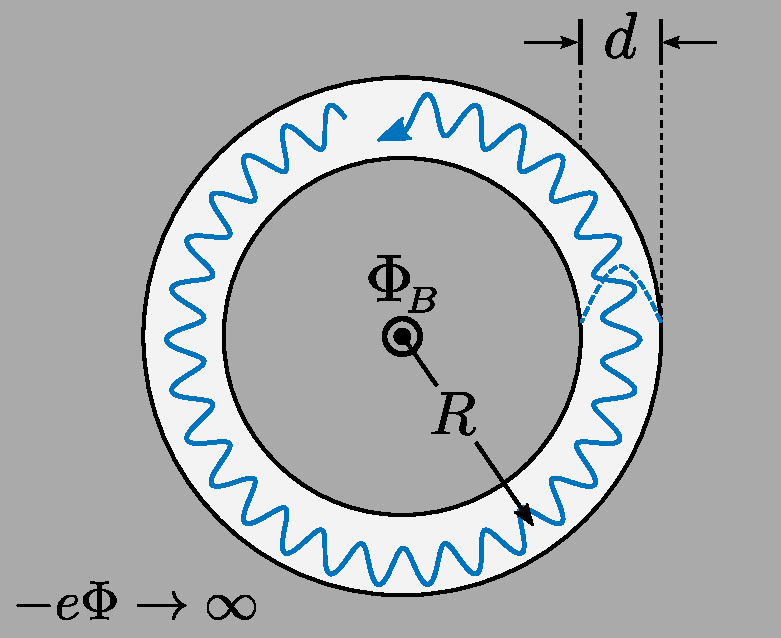
\includegraphics[width=0.65\textwidth]{annulus}
\end{figure}

\noindent
We assume all fields and wavefunctions to be independent of $z$ (the
out-of-plane direction).  The in-plane position can be expressed using
polar coordinates $(r,\phi)$, such that the annulus is centered at the
coordinate origin.

Suppose we use an infinitesimally thin solenoid to thread a magnetic
flux $\Phi_B$ through the origin.  This can be described by the vector
potential
\begin{equation}
  \mathbf{A}(r,\phi) = \frac{\Phi_B}{2\pi r} \, \mathbf{e}_\phi,
  \label{Asolenoid}
\end{equation}
where $\mathbf{e}_\phi$ is the unit vector pointing in the azimuthal
direction.  With this choice of $\mathbf{A}$ field, the magnetic flux
through a loop of radius $r$ around the origin is
\begin{equation}
  \oint \mathbf{A} \cdot d\mathbf{r} = \left(\frac{\Phi_B}{2\pi r}\right)
  \cdot (2\pi r)
  = \Phi_B,
\end{equation}
independent of $r$.  Thus, the magnetic flux density is entirely
concentrated at the origin.  Away from the origin, we have $\mathbf{A}
\ne 0$ and $\mathbf{B} = 0$.

Plugging this $\mathbf{A}$ field into the Hamiltonian
\eqref{timeindep}, we arrive at the time-independent Schr\"odinger
wave equation
\begin{equation}
  \frac{1}{2m}\left|-i\hbar\nabla+
  \frac{e\Phi_B}{2\pi r} \, \mathbf{e}_\phi\right|^2 \psi(r,\phi)
  = E\psi(r,\phi).
  \label{ABschrod}
\end{equation}
Due to rotational symmetry, the eigenfunctions should have the form
\begin{equation}
  \psi(r,\phi) = \psi_0 \, A(r)\, e^{in\phi}, \quad n \in \mathbb{Z}.
  \label{abansatz}
\end{equation}

Since the annulus is very thin ($d \ll R$), let us zoom in on a
representative local segment at $\phi = 0$, as shown below:

\begin{figure}[h]
  \centering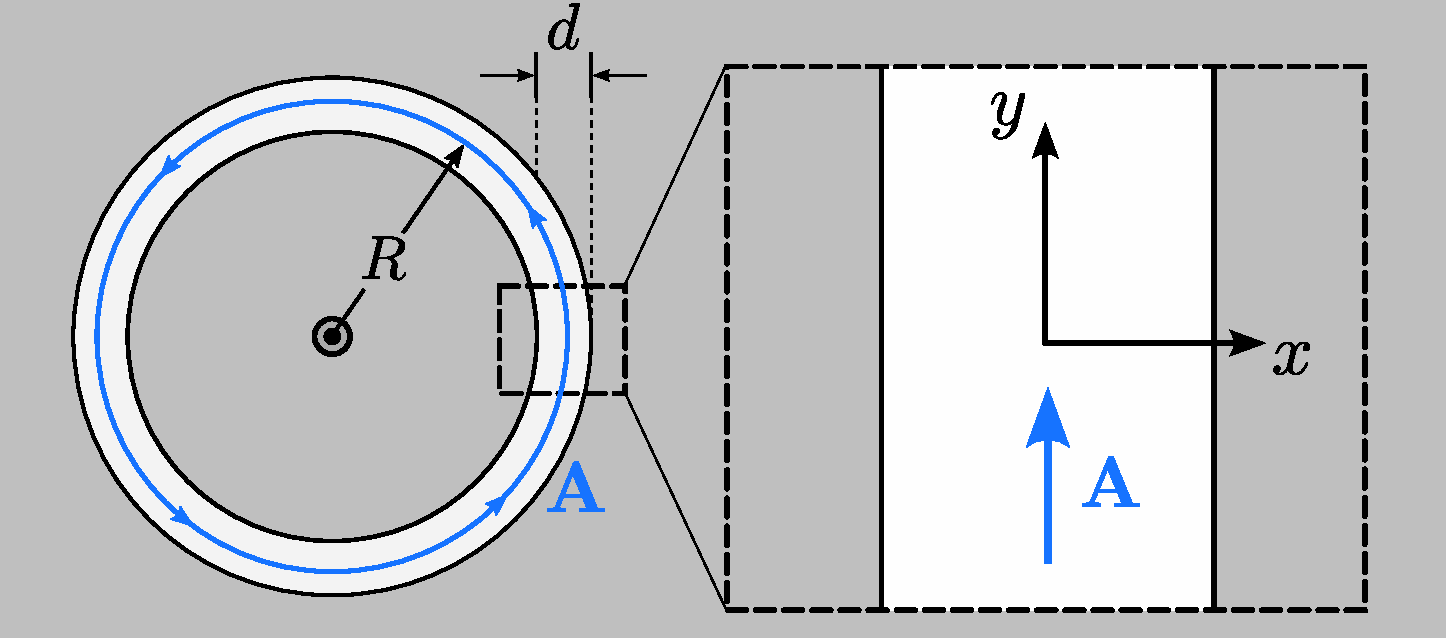
\includegraphics[width=0.62\textwidth]{annuluszoom}
\end{figure}

\noindent
Locally, the annulus looks like a straight waveguide.  Let us adopt
local Cartesian coordinates $x = r - R$ and $y = R\phi$.  Now
$\mathbf{A}$ points in the $y$ direction, so Eq.~\eqref{ABschrod}
reduces to
\begin{align}
  \left[-\frac{\hbar^2}{2m} \frac{\partial^2}{\partial x^2}
    + \frac{1}{2m} \left(-i\hbar \frac{\partial}{\partial y} +
    \frac{e\Phi_B}{2\pi R} \right)^2 \right] \psi(x, y) &\approx E \psi(x, y).
  \label{ABschrod2}
\end{align}
Meanwhile, the ansatz \eqref{abansatz} reduces to
\begin{equation}
  \psi(x,y) = A(x) e^{iny/R},
\end{equation}
which is a waveguide mode with transverse profile $A(x)$ and
wavenumber $k_y = n/R$.  This allows us to substitute
$\partial/\partial y \rightarrow in/R$ in Eq.~\eqref{ABschrod2},
giving
\begin{equation}
  \left[-\frac{\hbar^2}{2m} \frac{\partial^2}{\partial x^2} +
    \frac{1}{2m} \left(\frac{n\hbar}{R} +
    \frac{e\Phi_B}{2\pi R} \right)^2 \right] A(x) = E A(x).
  \label{ABschrod3}
\end{equation}
Since the wavefunction vanishes on the inner and outer walls of the
annulus, the transverse profile must satisfy
\begin{equation}
  A(\pm d/2) = 0. \label{rboundcond} 
\end{equation}
We pick the solution $A(x) = \cos(\pi x / d)$, which corresponds to
the fundamental waveguide mode.  Applying this to
Eq.~\eqref{ABschrod3} yields
\begin{align}
  E &= \frac{1}{2m} \left[
    \left(\frac{n\hbar}{R} + \frac{e\Phi_B}{2\pi R}\right)^2
    + \left(\frac{\pi\hbar}{d}\right)^2 \right] \\
  &= \frac{e^2}{8\pi^2mR^2} \left(\Phi_B + \frac{nh}{e} \right)^2
  + \frac{\pi^2\hbar^2}{2md^2}.
  \label{abcurves}
\end{align}
There is an infinite set of solutions, indexed by $n \in \mathbb{Z}$.
For each $n$, the energy varies quadratically with the magnetic flux
$\Phi_B$, with an $n$-dependent $\Phi_B$ offset and a constant energy
offset.  The spectrum is plotted against $\Phi_B$ below:

\begin{figure}[h]
  \centering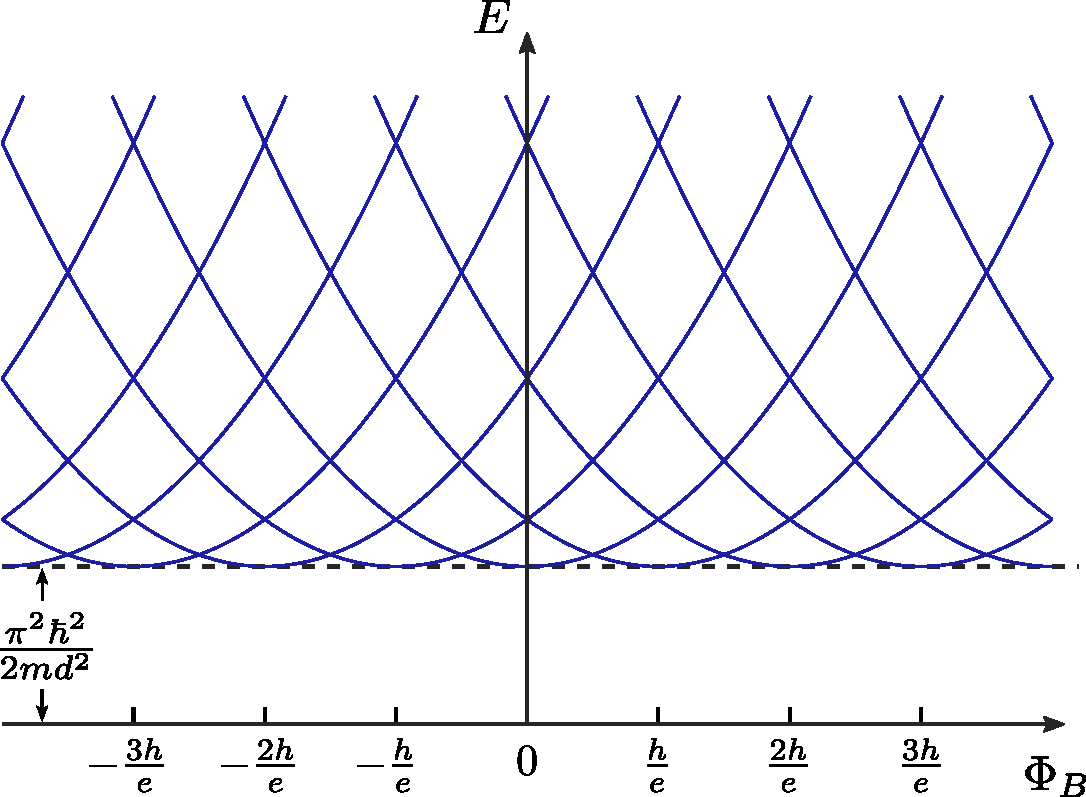
\includegraphics[width=0.58\textwidth]{abring}
\end{figure}

Evidently, varying $\Phi_B$ affects the energy eigenvalues, in spite
of the fact that the electron resides in the annulus where $\mathbf{B}
= 0$.  This is the Aharonov-Bohm effect.

A further noteworthy feature of this spectrum is that if $\Phi_B$
changes by a multiple of the constant $h/e$ (called the
\textbf{magnetic flux quantum}), the spectrum is left unchanged.  This
invariance property turns out to be tied to gauge symmetry.
Eq.~\eqref{Asolenoid} says that if an extra flux $nh/e$ (where
$n\in\mathbb{Z}$) is threaded through the annulus, the vector
potential changes by $\Delta \mathbf{A} = (n\hbar/ e r)
\mathbf{e}_\phi$.  But we can undo this via the following gauge
transformation:
\begin{equation}
  \Lambda(r,\phi) = - \frac{n\hbar}{e} \, \phi \;\;\;\Rightarrow
  \begin{cases}\nabla \Lambda &= \displaystyle - (n\hbar/er) \, \mathbf{e}_\phi
    \\ \displaystyle e^{-ie\Lambda/\hbar} &= \displaystyle e^{in\phi}.
  \end{cases}
\end{equation}
Note that $\Lambda$ is not single-valued, but that's not a problem, as
both $\nabla\Lambda$ and $\exp(-ie\Lambda/\hbar)$, which enter into
the gauge symmetry relations \eqref{Hlambda}--\eqref{gaugepsi}, are
single-valued.

Remarkably, this gauge argument does not require the electron to live
on an annulus; we can consider a confinement region of any shape, so
long as it encircles the magnetic flux.  In general, the energy
spectrum need not be given by Eq.~\eqref{abcurves}, but the gauge
argument says that it must be invariant under a flux change of $\Delta
\Phi_B = n h/e$.

This invariance property is also closely related to a famous argument
by Dirac, showing that if there exists a magnetic monopole---a
hypothetical particle that produces a magnetic field $\mathbf{B} =
(\mu/4\pi r^2)\, \mathbf{e}_r$---then its magnetic charge $\mu$ must
be a multiple of $h/e$.  Conversely, if there exists a single magnetic
monopole of charge $\mu$ anywhere in the universe, electric charges
must come in multiples of $h/\mu$, which could be regarded as an
explanation for the quantization of electric charge
[\ref{cite:monopole}].

\section{Dirac's Theory of the Electron}

\subsection{The Dirac Hamiltonian}
\label{sec:DiracH}

So far, we have been using $p^2/2m$-type Hamiltonians, which are
limited to describing non-relativistic particles.  In 1928, Paul Dirac
formulated a Hamiltonian that can describe electrons moving close to
the speed of light, thus successfully combining quantum theory with
special relativity. Another triumph of Dirac's theory is that it
accurately predicts the magnetic moment of the electron.

Dirac's theory begins from the time-dependent Schr\"odinger wave
equation,
\begin{equation}
  i\hbar\, \partial_t\, \psi(\mathbf{r},t)
  = \hat{H} \psi(\mathbf{r},t).
  \label{schrod}
\end{equation}
Note that the left side has a first-order time derivative.  On the
right, the Hamiltonian $\hat{H}$ contains spatial derivatives in the
form of momentum operators.  We know that time and space derivatives
of the wavefunction are related to energy and momentum, respectively:
\begin{equation}
    i\hbar\, \partial_t\; \leftrightarrow \;
    E, \qquad
    -i\hbar\, \partial_j \;\leftrightarrow \;
    p_j.
\end{equation}
We also know that the energy and momentum of a relativistic particle
are related by
\begin{equation}
  E^2 = m^2c^4 + \sum_{j=1}^3 p_j^2c^2,
  \label{Erelativistic}
\end{equation}
where $m$ is the rest mass and $c$ is the speed of light.  (Following
the usual practice in relativity theory, we use Roman indices $j \in
\{1,2,3\}$ for the spatial coordinates $\{x,y,z\}$.)

Since the left side of Eq.~\eqref{schrod} has a first-order time
derivative, we guess that the Hamiltonian on the right should involve
first-order spatial derivatives.  Let us take
\begin{equation}
  \hat{H} = \alpha_0 mc^2 + \sum_{j=1}^3 \alpha_j \hat{p}_j c,
  \label{Dirac0}
\end{equation}
where $\hat{p}_j \equiv -i\hbar \partial_j$.  The $mc^2$ and $c$
factors are placed for later convenience.  To determine the
dimensionless ``coefficients'' $\alpha_0$, $\alpha_1$, $\alpha_2$, and
$\alpha_3$, consider a wavefunction with definite energy $E$ and
momentum $\mathbf{p}$:
\begin{equation}
  \left\{\begin{aligned}\hat{H}\psi &= E \psi \\
  \hat{p}_i \psi &= p_i \psi
  \end{aligned}\right.
    \;\;\;\Rightarrow \;\;\;
  \left(\alpha_0mc^2 + \sum_{j=1}^3\alpha_j p_jc\right) \psi = E\,\psi.
\end{equation}
If $\psi$ is a scalar, this would imply that
\begin{equation*}
  \alpha_0 mc^2 + \sum_{j}\alpha_j p_j c = E
\end{equation*}
for certain scalar coefficients $\{\alpha_0, \dots, \alpha_3\}$, which
does not match Eq.~\eqref{Erelativistic} at all!

But we can get things to work if $\psi(\mathbf{r},t)$ is a
multi-component wavefunction, rather than a scalar wavefunction, and
the $\alpha$'s are matrices acting on those components via the
matrix-vector product operation.  In that case,
\begin{framed}
  \begin{equation}
    \hat{H} = \hat{\alpha}_0 mc^2 + \sum_{j=1}^3 \hat{\alpha}_j \hat{p}_j c,
    \;\; \mathrm{where}\;\; \hat{p}_j \equiv -i\hbar\, \partial_j,
    \label{Dirac}
  \end{equation}
\end{framed}
\vskip -0.05in
\noindent
where the hats on $\{\hat{\alpha}_0, \dots, \hat{\alpha}_3\}$ indicate
that they are matrix-valued.  Applying the Hamiltonian twice gives
\begin{equation}
  \Big(\hat{\alpha}_0mc^2 + \sum_{j}\hat{\alpha}_j p_j c\Big)^{\!2}\;
  \psi = E^2\,\psi.
\end{equation}
This can be satisfied if
\begin{equation}
  \Big(\hat{\alpha}_0 mc^2 + \sum_{j}\hat{\alpha}_j p_j c\Big)^2
  = E^2\, \hat{I},
\end{equation}
where $\hat{I}$ is the identity matrix.  Expanding the square (and
taking care of the fact that the $\hat{\alpha}_\mu$ matrices need not
commute) yields
\begin{equation}
  \hat{\alpha}_0^2 m^2c^4
  + \sum_j \left(\hat{\alpha}_0 \hat{\alpha}_j + \hat{\alpha}_j \hat{\alpha}_0\right) mc^3 p_j
  + \sum_{jj'} \hat{\alpha}_j \hat{\alpha}_{j'} \, p_j p_{j'} \,c^2 = E^2\hat{I}.
\end{equation}
This reduces to Eq.~\eqref{Erelativistic} if the $\hat{\alpha}_\mu$
matrices satisfy
\begin{align}
  \begin{aligned}
    \hat{\alpha}_\mu^2 &= \hat{I} \;\;\; \textrm{for} \;\;\mu=0,1,2,3,
    \;\;\textrm{and} \\
    \hat{\alpha}_\mu \hat{\alpha}_\nu
    + \hat{\alpha}_\nu \hat{\alpha}_\mu &= 0
    \;\;\; \textrm{for} \;\;\mu \ne \nu.
  \end{aligned}
\end{align}
(We use Greek symbols for indices ranging over the four spacetime
coordinates $\{0,1,2,3\}$.)  The above can be written more concisely
using the anticommutator:
\begin{equation}
  \{\hat{\alpha}_\mu, \hat{\alpha}_\nu\} = 2\delta_{\mu\nu},
  \;\;\; \textrm{for} \;\;\mu,\nu=0,1,2,3.
  \label{Dirac_anticomm}
\end{equation}
Also, we need the $\hat{\alpha}_\mu$ matrices to be Hermitian, so that
$\hat{H}$ is Hermitian.

It turns out that the smallest possible Hermitian matrices that can
satisfy Eq.~\eqref{Dirac_anticomm} are $4\times4$ matrices.  The
choice of matrices (or ``representation'') is not uniquely determined.
One particularly useful choice is called the \textbf{Dirac
  representation}:
\begin{align}
  \begin{aligned}
    \hat{\alpha}_0 &= \begin{bmatrix}
      \hat{I}\, & \hat{0} \\ \hat{0} & -\hat{I}
    \end{bmatrix}, \;\;\;
    \hat{\alpha}_1 = \begin{bmatrix}
      \hat{0} & \hat{\sigma}_1 \\ \hat{\sigma}_1 & \hat{0}
    \end{bmatrix} \\
    \hat{\alpha}_2 &= \begin{bmatrix}
      \hat{0} & \hat{\sigma}_2 \\ \hat{\sigma}_2 & \hat{0}
    \end{bmatrix}, \;\;\;
    \hat{\alpha}_3 = \begin{bmatrix}
      \hat{0} & \hat{\sigma}_3 \\ \hat{\sigma}_3 & \hat{0}
    \end{bmatrix},
  \end{aligned}
  \label{alpha_matrices}
\end{align}
where $\{\hat{\sigma}_{1}, \hat{\sigma}_{2}, \hat{\sigma}_{3}\}$
denote the usual Pauli matrices.  Since the $\hat{\alpha}_\mu$'s are
$4\times4$ matrices, it follows that $\psi(\mathbf{r})$ is a
four-component field.

\subsection{Eigenstates of the Dirac Hamiltonian}
\label{sec:deigenstates}

According to Eq.~\eqref{Erelativistic}, the energy eigenvalues of the
Dirac Hamiltonian are
\begin{equation}
  E = \pm \sqrt{m^2c^4 + \sum_{j} p_j^2c^2}.
\end{equation}
This is plotted below:

\begin{center}
  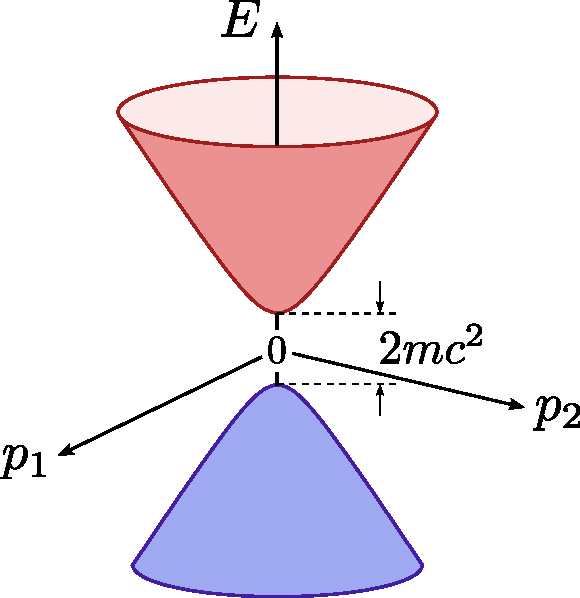
\includegraphics[width=0.27\textwidth]{diraccone}
\end{center}

\noindent
The energy spectrum forms two hyperbolas.  The upper hyperbola matches
the standard dispersion relation for a massive relativistic particle.
But what about the negative-energy hyperbola?  Who ordered that?

If we are considering an isolated electron, it might be possible for
us to simply declare that we are only interested in the
positive-energy states, and ignore the negative-energy states.
However, this becomes untenable once we couple the electron to
additional systems like the electromagnetic field: even if the
electron starts with $E > 0$, it can hop to the negative-energy
hyperbola by shedding energy into the external system.  This seems
like a glaring problem, but let us wait till
Section~\ref{sec:positrons} to discuss how to resolve it.

Moreover, each hyperbola is two-fold degenerate.  Since the Dirac
wavefunction has four components, for each $\mathbf{p}$ there are four
orthogonal energy eigenstates, two with (equal) positive energy and
two with (equal) negative energy.  However, the four wavefunction
components are \textit{not} necessarily related in a simple way to the
choice of positive or negative $E$.  Let us take the Dirac
representation \eqref{alpha_matrices}, and divide the components by
\begin{equation}
  \psi(\mathbf{r},t) = \begin{bmatrix}\psi_A(\mathbf{r},t)
    \\ \psi_B(\mathbf{r},t)
  \end{bmatrix},
  \label{diracdivision}
\end{equation}
where $\psi_A$ and $\psi_B$ have two components each.  The Dirac
equation \eqref{Dirac} then reduces to
\begin{align}
  \psi_A &= \frac{1}{E - mc^2} \sum_j \hat{\sigma}_j p_j \psi_B,
  \label{dirac_nonrel1} \\
  \psi_B &= \frac{1}{E + mc^2} \sum_j \hat{\sigma}_j p_j \psi_A.
  \label{dirac_nonrel2}
\end{align}
For $|\mathbf{p}| \rightarrow 0$, $E$ approaches either $mc^2$ or
$-mc^2$.  On the upper hyperbola ($E \sim mc^2$), the vanishing of the
denominator in Eq.~\eqref{dirac_nonrel1} implies that the wavefunction
is dominated by $\psi_A$, with $\psi_B \sim 0$.  Conversely, on the
lower hyperbola ($E \sim -mc^2$), the wavefunction is dominated by
$\psi_B$, with $\psi_A \sim 0$.

However, this association only holds in the non-relativistic limit!
In the relativistic regime, $|\mathbf{p}| \sim |E| \gg mc^2$,
Eqs.~\eqref{dirac_nonrel1} and \eqref{dirac_nonrel2} imply that
$|\psi_A| \sim |\psi_B|$ for both positive-energy and negative-energy
eigenstates.  (There does exist a way to make the upper/lower
components correspond rigorously to positive/negative $E$, but this
requires adopting a much more complicated matrix representation
[\ref{cite:foldy}].)

In the next section, we will see that the two-fold degeneracy of each
energy hyperbola is related to the electron's spin degree of freedom.

\subsection{Dirac electron in an electromagnetic field}
\label{sec:diracem}

Let us next look at how Dirac's electron interacts with an
electromagnetic field.  To introduce the electromagnetic field into
the theory, we follow the same procedure as in the non-relativistic
theory (Section~\ref{sec:nonrel}): add $-e\Phi(\mathbf{r},t)$ as a
scalar potential function, and add the vector potential via the
substitution
\begin{equation}
  \hat{\mathbf{p}} \rightarrow \hat{\mathbf{p}}
  + e\mathbf{A}(\hat{\mathbf{r}},t).  
\end{equation}
Applying this recipe to the Dirac Hamiltonian (\ref{Dirac}) yields
\begin{equation}
  i\hbar \, \partial_t \psi
  = \left\{\hat{\alpha}_0 mc^2 -e\Phi(\mathbf{r},t)
  + \sum_{j} \hat{\alpha}_j \Big[-i\hbar\,\partial_j
    +eA_j(\mathbf{r},t) \Big] c\right\}\psi(\mathbf{r},t).
  \label{DiracEM}
\end{equation}
You can check that this has the same gauge symmetry properties as the
non-relativistic theory discussed in Section~\ref{sec:gauge}.

We now take the Dirac representation \eqref{alpha_matrices}.
Moreover, following Eq.~\eqref{diracdivision}, let $\psi_A$ and
$\psi_B$ denote the the Dirac wavefunction's upper and lower
components (each having two components).  Then Eq.~\eqref{DiracEM}
reduces to
\begin{align}
  i\hbar\, \partial_t \, \psi_A
  &= \big(+mc^2 -e\Phi \big)\,
  \psi_A
  \,+\, \sum_{j} \hat{\sigma}_j \big(-i\hbar\partial_j
    +eA_j \big) \,c\;\psi_B \label{Dirac2a} \\
  i\hbar\, \partial_t \, \psi_B
  &= \big(- mc^2 -e\Phi\big)\,
  \psi_B \,+\, \sum_{j} \hat{\sigma}_j \big(-i\hbar\partial_j
    +eA_j \big)\, c\;\psi_A, \label{Dirac2b}
\end{align}
In the non-relativistic limit, we can seek solutions of the form
\begin{align}
  \begin{aligned}
  \psi_{A/B}(\mathbf{r},t) &= \Psi_{A/B}(\mathbf{r},t)\,
  \exp\left[-i\left(\frac{mc^2}{\hbar}\right)t\right].
  \end{aligned}
\end{align}
The phase factor on the right side comes from the rest energy $mc^2$.
This is assumed to be by far the largest energy scale in the problem,
corresponding to a fast oscillation.  (By using $mc^2$ rather than
$-mc^2$, we are focusing on the positive-energy states.)  The
functions $\Psi_A$ and $\Psi_B$ are ``slowly-varying envelopes'',
which have $t$-dependences much slower than the phase factor.  When
$\mathbf{p} = 0$ and $\Phi = \mathbf{A} = 0$, they reduce to
constants.

Plugging this ansatz into Eqs.~\eqref{Dirac2a}--\eqref{Dirac2b} gives
\begin{align}
  i\hbar\, \partial_t \, \Psi_A
  &= -e\Phi\; \Psi_A
  \,+\, \sum_{j} \hat{\sigma}_j \big(-i\hbar\partial_j
    +eA_j \big) c\;\Psi_B \label{Dirac3a} \\
  \big(i\hbar\, \partial_t \, + 2mc^2 + e\Phi\big)
  \Psi_B
  &= \sum_{j} \hat{\sigma}_j \big(-i\hbar\partial_j
    +eA_j \big) c\;\Psi_A. \label{Dirac3b}
\end{align}
On the left side of Eq.~\eqref{Dirac3b}, the $2mc^2$ term dominates
over the other two, so
\begin{equation}
  \Psi_B \;\approx\; \frac{1}{2mc}\, \sum_{j}
  \hat{\sigma}_j \big(-i\hbar\partial_j +eA_j \big) \;\Psi_A.
\end{equation}
Plugging this into Eq.~\eqref{Dirac3a} yields
\begin{equation}
  i\hbar\, \partial_t \, \Psi_A
  = \left\{-e\Phi \,+\, \frac{1}{2m} \sum_{jk} \hat{\sigma}_j \hat{\sigma}_k
  \big(-i\hbar\partial_j +eA_j \big)
  \big(-i\hbar\partial_k +eA_k \big) \right\}\;\Psi_A.
\end{equation}
Using the identity $\hat{\sigma}_j\hat{\sigma}_k = \delta_{jk}\hat{I}
+ i \sum_i \varepsilon_{ijk}\sigma_i$:
\begin{align}
  \begin{aligned}
  i\hbar\, \partial_t \, \Psi_A
  &= \Bigg\{-e\Phi
  \,+\, \frac{1}{2m} \big|-i\hbar\nabla +e\mathbf{A} \big|^2 \\
  &\qquad+\, \frac{i}{2m} \sum_{ijk} \varepsilon_{ijk} \hat{\sigma}_i
  \big(-i\hbar\partial_j +eA_j \big)
  \big(-i\hbar\partial_k +eA_k \big)
  \Bigg\} \Psi_A.
  \end{aligned}
\end{align}
Look carefully at the last term in the curly brackets.  Expanding the
square yields
\begin{equation*}
  \frac{i}{2m}\sum_{ijk}\varepsilon_{ijk}\hat{\sigma}_i
  \Big(-\partial_j\partial_k -i\hbar e \partial_jA_k
  - i\hbar e \big[A_k\partial_j + A_j\partial_k \big]
  + e^2A_jA_k \Big).
\end{equation*}
Due to the antisymmetry of $\varepsilon_{ijk}$, all terms inside the
parentheses that are symmetric under $j$ and $k$ cancel out when
summed over.  The only survivor is the second term, which gives
\begin{equation}
  \frac{\hbar e}{2m}\sum_{ijk}\varepsilon_{ijk}\hat{\sigma}_i
  \partial_jA_k = \frac{\hbar e}{2m} \hat{\boldsymbol{\sigma}}
  \,\cdot\, \mathbf{B}(\mathbf{r},t),
\end{equation}
where $\mathbf{B} = \nabla\times\mathbf{A}$ is the magnetic field.
Hence,
\begin{equation}
  i\hbar\, \partial_t \, \Psi_A
  = \left\{-e\Phi
  \,+\, \frac{1}{2m} \big|-i\hbar\nabla +e\mathbf{A} \big|^2
  \,-\, \left(-\frac{\hbar e}{2m}\, \hat{\boldsymbol{\sigma}}\right)
  \,\cdot\, \mathbf{B} \right\} \Psi_A.
\end{equation}
On the right side, we see the Hamiltonian for a non-relativistic
electron in an electromagnetic field, Eq.~\eqref{quantumH}, but with
an additional term of the form $- \hat{\boldsymbol{\mu}} \cdot
\hat{\mathbf{B}}$.  This new term matches the potential energy of a
magnetic dipole of moment $\boldsymbol{\mu}$ in a magnetic field
$\mathbf{B}$.  Therefore, the theory predicts that the electron has a
magnetic dipole moment of
\begin{equation}
  |\boldsymbol{\mu}| = \frac{\hbar e}{2m}.
  \label{Diracmu}
\end{equation}
Remarkably, this matches the experimentally-observed magnetic dipole
moment to about one part in $10^3$.  The residual mismatch between
Eq.~\eqref{Diracmu} and the actual magnetic dipole moment of the
electron is understood to arise from quantum fluctuations of the
electronic and electromagnetic quantum fields.  Using the full theory
of quantum electrodynamics, that ``anomalous magnetic moment'' can
also be calculated and matches experiment to around one part in
$10^9$, making it one of the most precise theoretical predictions in
physics [\ref{cite:zee}]!

It is noteworthy that we did not set out to include spin in the
theory, yet it arose, seemingly unavoidably, as a by-product of
formulating a relativistic theory of the electron.  This is a
manifestation of the principle that relativistic quantum theory is
more constrained than non-relativistic quantum
theory~[\ref{cite:dyson}].  To satisfy the relativistic symmetries,
spin cannot be an optional part of the theory---it must be built-in at
a fundamental level.

\subsection{Positrons and Dirac Field Theory}
\label{sec:positrons}

As noted in Section~\ref{sec:deigenstates}, the stability of the
quantum states described by the Dirac equation is threatened by the
presence of negative-energy solutions.  To get around this problem,
Dirac suggested that what we regard as the ``vacuum'' may actually be
a state, called the \textbf{Dirac sea}, in which all negative-energy
states are occupied.  Since electrons are fermions, the Pauli
exclusion principle would then forbid decay into the negative-energy
states, stabilizing the positive-energy states.

At first blush, the idea seems ridiculous; how can the vacuum contain
an infinite number of particles?  However, we shall see that the idea
becomes more plausible if the Dirac equation is reinterpreted as a
single-particle \textit{construction} which arises from a more
fundamental quantum field theory.  The Dirac sea idea is an inherently
multi-particle concept, and we know from Chapter 4 that quantum field
theory is a natural framework for describing multi-particle quantum
states.  Let us therefore develop this theory.

Consider again the eigenstates of the single-particle Dirac
Hamiltonian with definite momenta and energies.  Denote the
positive-energy wavefunctions by
\begin{equation}
  \frac{u_{\mathbf{k}\sigma} \, e^{i\mathbf{k}\cdot \mathbf{r}}}{(2\pi)^{3/2}}
  = \langle \mathbf{r} | \mathbf{k}, +, \sigma\rangle,
  \quad\mathrm{where}\;\;
  \hat{H} |\mathbf{k}, +, \sigma\rangle
  = \epsilon_{\mathbf{k}\sigma} |\mathbf{k}, +, \sigma\rangle.
  \label{Diraces1}
\end{equation}
The negative-energy wavefunctions are
\begin{equation}
  \frac{v_{\mathbf{k}\sigma} \, e^{-i\mathbf{k}\cdot \mathbf{r}}}{(2\pi)^{3/2}}
  = \langle \mathbf{r} | \mathbf{k}, -, \sigma\rangle,
  \quad\mathrm{where}\;\;
  \hat{H} |\mathbf{k}, -, \sigma\rangle
  = - \epsilon_{\mathbf{k}\sigma} |\mathbf{k}, -, \sigma\rangle.
  \label{Diraces2}
\end{equation}
Note that $|\mathbf{k}, -, \sigma\rangle$ denotes a negative-energy
eigenstate with momentum $-\hbar\mathbf{k}$, not $\hbar\mathbf{k}$.
The reason for this notation, which uses different symbols to label
the positive-energy and negative-energy states, will become clear
later.  Each of the $u_{\mathbf{k}\sigma}$ and $v_{\mathbf{k}\sigma}$
terms are four-component objects (spinors), and for any given
$\mathbf{k}$, the set
\begin{equation*}
  \{ u_{\mathbf{k}\sigma}, v_{\mathbf{k},\sigma}\;\;  | \;\; \sigma = 1,2  \}
\end{equation*}
forms an orthonormal basis for the four-dimensional spinor space.
Thus,
\begin{equation}
  \sum_{n} \left(u^n_{\mathbf{k}\sigma}\right)^* u^n_{\mathbf{k}\sigma'} = \delta_{\sigma\sigma'}, \;\;
  \sum_{n} \left(u^n_{\mathbf{k}\sigma}\right)^* v^n_{\mathbf{k}\sigma'} = 0, \;\;
  \textrm{etc.}
  \label{uvorthog}
\end{equation}
Here we use the notation where $u^n_{\mathbf{k}\sigma}$ is the $n$-th
component of the $u_{\mathbf{k}\sigma}$ spinor, and likewise for the
$v$'s.

Following the second quantization procedure from Chapter 4, let us
introduce a fermionic Fock space $\mathscr{H}_F$, as well as a set of
creation/annihilation operators:
\begin{align*}
  \hat{b}_{\mathbf{k}\sigma}^\dagger \;\; \mathrm{and} \;\; \hat{b}_{\mathbf{k}\sigma}
  &\;\;\mathrm{create/annihilate} \;\; |\mathbf{k}, +, \sigma\rangle\\
  \hat{d}_{\mathbf{k}\sigma}^\dagger \;\; \mathrm{and} \;\; \hat{d}_{\mathbf{k}\sigma}
  &\;\;\mathrm{create/annihilate} \;\; |\mathbf{k}, -, \sigma\rangle.
\end{align*}
These obey the fermionic anticommutation relations
\begin{align}
  \begin{aligned}
    \{\hat{b}_{\mathbf{k}\sigma}, \hat{b}_{\mathbf{k}'\sigma'}^\dagger \}
    = \delta^3(\mathbf{k}-\mathbf{k}') \, \delta_{\sigma\sigma'}, \quad
    \{\hat{d}_{\mathbf{k}\sigma}, \hat{d}_{\mathbf{k}'\sigma'}^\dagger \}
    = \delta^3(\mathbf{k}-\mathbf{k}') \, \delta_{\sigma\sigma'} \\
    \{\hat{b}_{\mathbf{k}\sigma}, \hat{b}_{\mathbf{k}'\sigma'} \} = 
    \{\hat{b}_{\mathbf{k}\sigma}, \hat{d}_{\mathbf{k}'\sigma'} \} = 
    \{\hat{d}_{\mathbf{k}\sigma}, \hat{d}_{\mathbf{k}'\sigma'} \} = 0, \;\;\textrm{etc.}
  \end{aligned}
  \label{Diracanticommutation0}
\end{align}
The Hamiltonian is
\begin{equation}
  \hat{H} = \int d^3k \sum_\sigma \epsilon_{\mathbf{k}\sigma} \left(
  \hat{b}^\dagger_{\mathbf{k}\sigma} \hat{b}_{\mathbf{k}\sigma}
  - \hat{d}^\dagger_{\mathbf{k}\sigma} \hat{d}_{\mathbf{k}\sigma}
  \right),
  \label{HDiracQFT0}
\end{equation}
and applying the annihilation operators to the vacuum state
$|\varnothing\rangle$ gives zero:
\begin{equation}
  \hat{b}_{\mathbf{k}\sigma} |\varnothing\rangle =
  \hat{d}_{\mathbf{k}\sigma} |\varnothing\rangle = 0.
\end{equation}

When formulating bosonic field theory, we defined a local field
annihilation operator that annihilates a particle at a given point
$\mathbf{r}$.  In the infinite-system limit, this took the form
\begin{equation}
  \hat{\psi}(\mathbf{r})
  = \int d^3k \; \varphi_{\mathbf{k}}(\mathbf{r}) \, \hat{a}_{\mathbf{k}},
\end{equation}
and the orthonormality of the $\varphi_{\mathbf{k}}$ wavefunctions
implied that $[\hat{\psi}(\mathbf{r}),
  \hat{\psi}^\dagger(\mathbf{r}')] =
\delta^3(\mathbf{r}-\mathbf{r}')$.  Similarly, we can use the Dirac
Hamiltonian's eigenfunctions \eqref{Diraces1}--\eqref{Diraces2} to
define
\begin{equation}
  \hat{\psi}_n(\mathbf{r})
  = \int \frac{d^3k}{(2\pi)^{3/2}} \; \sum_\sigma
  \left(
  u^n_{\mathbf{k}\sigma} e^{i\mathbf{k}\cdot\mathbf{r}} \, \hat{b}_{\mathbf{k}\sigma}
  + v^n_{\mathbf{k}\sigma} e^{-i\mathbf{k}\cdot\mathbf{r}} \, \hat{d}_{\mathbf{k}\sigma}\right).
  \label{Diracpsi0}
\end{equation}
Note that there are two terms in the parentheses because the
positive-energy and negative-energy states are denoted by
differently-labeled annihilation operators.  Moreover, since the
wavefunctions are four-component spinors, the field operators have a
spinor index $n$.  Using the spinor orthonormality conditions
\eqref{uvorthog} and the anticommutation relations
\eqref{Diracanticommutation0}, we can show that
\begin{equation}
  \left\{\hat{\psi}_n(\mathbf{r}), \hat{\psi}_{n'}^{\dagger}(\mathbf{r}')\right\}
  = \delta_{nn'}\, \delta^3(\mathbf{r}-\mathbf{r}'),
\end{equation}
with all other anticommutators vanishing.  Hence,
$\hat{\psi}_n(\mathbf{r})$ can be regarded as an operator that
annihilates a four-component fermion at point $\mathbf{r}$.

Now let us \textit{define} the operators
\begin{equation}
  \hat{c}_{\mathbf{k}\sigma} = \hat{d}^\dagger_{\mathbf{k}\sigma}.
\end{equation}
Using these, the fermionic anticommutation relations can be re-written as
\begin{align}
  \begin{aligned}
    \{\hat{b}_{\mathbf{k}\sigma}, \hat{b}_{\mathbf{k}'\sigma'}^\dagger \}
    = \delta^3(\mathbf{k}-\mathbf{k}') \, \delta_{\sigma\sigma'}, \quad
    \{\hat{c}_{\mathbf{k}\sigma}, \hat{c}_{\mathbf{k}'\sigma'}^\dagger \}
    = \delta^3(\mathbf{k}-\mathbf{k}') \, \delta_{\sigma\sigma'} \\
    \{\hat{b}_{\mathbf{k}\sigma}, \hat{b}_{\mathbf{k}'\sigma'} \} = 
    \{\hat{b}_{\mathbf{k}\sigma}, \hat{c}_{\mathbf{k}'\sigma'} \} = 
    \{\hat{c}_{\mathbf{k}\sigma}, \hat{c}_{\mathbf{k}'\sigma'} \} = 0, \;\;\textrm{etc.}
  \end{aligned}
  \label{Diracanticommutators}
\end{align}
Hence $\hat{c}^\dagger_{\mathbf{k}\sigma}$ and
$\hat{c}_{\mathbf{k}\sigma}$ formally satisfy the criteria to be
regarded as creation and annihilation operators.  The particle created
by $\hat{c}^\dagger_{\mathbf{k}\sigma}$ is called a \textbf{positron},
and is equivalent to the \textit{absence} of a $d$-type particle
(i.e., a negative-energy electron).

The Hamiltonian \eqref{HDiracQFT0} can now be written as
\begin{equation}
  \hat{H} = \int d^3k \sum_\sigma \epsilon_{\mathbf{k}\sigma} \left(
  \hat{b}^\dagger_{\mathbf{k}\sigma} \hat{b}_{\mathbf{k}\sigma}
  + \hat{c}^\dagger_{\mathbf{k}\sigma} \hat{c}_{\mathbf{k}\sigma}
  \right) \;\; + \;\; \textrm{constant},
  \label{HDiracQFT}
\end{equation}
which explicitly shows that the positrons have positive energies
(i.e., the absence of a negative-energy particle is equivalent to the
presence of a positive-energy particle).  With further analysis, which
we will skip, it can be shown that the positron created by
$\hat{c}^\dagger_{\mathbf{k}\sigma}$ has positive charge $e$ and
momentum $\hbar\mathbf{k}$.  The latter is thanks to the definition
adopted in Eq.~\eqref{Diraces2}; the absence of a momentum $-\hbar
\mathbf{k}$ particle is equivalent to the presence of a momentum
$\hbar \mathbf{k}$ particle.  As for the field annihilation operator
\eqref{Diracpsi0}, it can be written as
\begin{equation}
  \hat{\psi}_n(\mathbf{r})
  = \int \frac{d^3k}{(2\pi)^{3/2}} \; \sum_\sigma
  \left(
  u^n_{\mathbf{k}\sigma} e^{i\mathbf{k}\cdot\mathbf{r}} \, \hat{b}_{\mathbf{k}\sigma}
  + v^n_{\mathbf{k}\sigma} e^{-i\mathbf{k}\cdot\mathbf{r}} \,
  \hat{c}^\dagger_{\mathbf{k}\sigma}\right).
  \label{Diracpsi}
\end{equation}

The $c$-type annihilation operators do \textit{not} annihilate
$|\varnothing\rangle$.  However, let us define
\begin{equation}
  |\varnothing'\rangle = \prod_{\mathbf{k}\sigma} \hat{d}_{\mathbf{k}\sigma}^\dagger
  |\varnothing\rangle,
\end{equation}
which is evidently a formal description of the Dirac sea state.  Then
\begin{equation}
  \hat{c}_{\mathbf{k}\sigma} |\varnothing'\rangle = 
  \hat{d}^\dagger_{\mathbf{k}\sigma} \prod_{\mathbf{k}'\sigma'}
  \hat{d}_{\mathbf{k}'\sigma'}^\dagger |\varnothing\rangle = 0.
\end{equation}

At the end of the day, we can regard the quantum field theory as being
defined in terms of $b$-type and $c$-type operators, using the
anticommutators \eqref{Diracanticommutators}, the Hamiltonian
\eqref{HDiracQFT}, and the field operator \eqref{Diracpsi}, along with
the vacuum state $|\varnothing'\rangle$.  The elementary particles in
this theory are electrons and positrons with strictly positive
energies.  The single-particle Dirac theory, with its quirky
negative-energy states, can then be interpreted as a special construct
that maps the quantum field theory into single-particle language.
Even though we actually started from the single-particle description,
it is the quantum field theory, and its vacuum state
$|\varnothing'\rangle$, that is more fundamental.

There are many more details about the Dirac theory that we will not
discuss here.  One particularly important issue is how the particles
transform under Lorentz boosts and other changes in coordinate system.
For such details, the reader is referred to Ref.~[\ref{cite:dyson}].

\section{Quantizing the electromagnetic field}
\label{sec:em_quantization}

Previously (Chapter 4, Sec.~IV.C), we have gone through the process of
quantizing a scalar boson field.  The classical field is decomposed
into normal modes, and each mode is quantized by assigning it an
independent set of creation and annihilation operators.  By comparing
the oscillator energies in the classical and quantum regimes, we can
derive the Hermitian operator corresponding to the classical field
variable, expressed using the creation and annihilation operators.  We
will use the same approach, with only minor adjustments, to quantize
the electromagnetic field.

First, consider a ``source-free'' electromagnetic field---i.e., with
no electric charges and currents.  Without sources, Maxwell's
equations (in SI units, and in a vacuum) reduce to:
\begin{align}
  \nabla\cdot \mathbf{E} &= 0 \label{max1} \\
  \nabla\cdot \mathbf{B} &= 0 \label{max2}\\
  \nabla\times \mathbf{E} &= -\frac{\partial \mathbf{B}}{\partial t} \label{max3}\\
  \nabla\times \mathbf{B} &= \frac{1}{c^2} \frac{\partial \mathbf{E}}{\partial t}.
  \label{max4}
\end{align}
Once again, we introduce the scalar potential $\Phi$ and vector
potential $\mathbf{A}$:
\begin{align}
  \mathbf{E} &= - \nabla \Phi - \frac{\partial\mathbf{A}}{\partial t}
  \label{Efield} \\
  \mathbf{B} &= \nabla \times \mathbf{A}.
  \label{Bfield}
\end{align}
With these relations, Eqs.~\eqref{max2} and \eqref{max3} are satisfied
automatically via vector identities.  The two remaining equations,
\eqref{max1} and \eqref{max4}, become:
\begin{align}
  \nabla^2 \Phi &= -\frac{\partial}{\partial t} \nabla \cdot \mathbf{A} \label{max5} \\
  \left(\nabla^2 - \frac{1}{c^2}\frac{\partial^2}{\partial t^2}\right)
  \mathbf{A} &= \nabla\left[\frac{1}{c^2}\frac{\partial}{\partial t}  \Phi + \nabla\cdot\mathbf{A}\right]. \label{max6}
\end{align}

In the next step, we choose a convenient gauge called the
\textbf{Coulomb gauge}:
\begin{equation}
  \Phi = 0, \;\;\; \nabla \cdot \mathbf{A} = 0.
  \label{coulomb}
\end{equation}
(To see that we can always make such a gauge choice, suppose we start
out with a scalar potential $\Phi_0$ and vector potential
$\mathbf{A}_0$ not satisfying \eqref{coulomb}.  Perform a gauge
transformation with $\Lambda(\mathbf{r}, t) = - \int^t dt'\;
\Phi_0(\mathbf{r}, t')$.  The new scalar potential is $\Phi = \Phi_0 +
\dot{\Lambda} = 0$; moreover, the new vector potential satisfies
\begin{equation}
  \nabla\cdot\mathbf{A} = \nabla\cdot \mathbf{A}_0 - \nabla^2 \Lambda
  = \nabla\cdot \mathbf{A}_0 + \int^t dt'\; \nabla^2\Phi_0(\mathbf{r}, t').
\end{equation}
Upon using Eq.~\eqref{max5}, we find that $\nabla\cdot\mathbf{A} =
0$.)

In the Coulomb gauge, Eq.~\eqref{max5} is automatically satisfied.
The sole remaining equation, \eqref{max6}, simplifies to
\begin{equation}
  \left(\nabla^2 - \frac{1}{c^2}\frac{\partial^2}{\partial t^2}\right)
  \mathbf{A} = 0. \label{max8}
\end{equation}
This has plane-wave solutions of the form
\begin{equation}
  \mathbf{A}(\mathbf{r},t) = \Big(\mathcal{A}\, \,
  e^{i(\mathbf{k}\cdot\mathbf{r} - \omega t)} + \mathrm{c.c.}\Big)\,
  \mathbf{e},
  \label{lightplanewave}
\end{equation}
where $\mathcal{A}$ is a complex number (the \textbf{mode amplitude})
that specifies the magnitude and phase of the plane wave, $\mathbf{e}$
is a real unit vector (the \textbf{polarization vector}) that
specifies which direction the vector potential points along, and
``c.c.''~denotes the complex conjugate of the first term.  Referring
to Eq.~\eqref{max8}, the angular frequency $\omega$ must satisfy
\begin{equation}
  \omega = c|\mathbf{k}|.
\end{equation}
Moreover, since $\nabla \cdot \mathbf{A} = 0$, it must be the case
that
\begin{equation}
  \mathbf{k} \cdot \mathbf{e} = 0.
\end{equation}
In other words, the polarization vector is perpendicular to the
propagation direction.  For any given $\mathbf{k}$, we can choose
(arbitrarily) two orthogonal polarization vectors.

Now suppose we put the electromagnetic field in a box of volume $V =
L^3$, with periodic boundary conditions (we will take $L \rightarrow
\infty$ at the end).  The $\mathbf{k}$ vectors form a discrete set:
\begin{equation}
  k_j = \frac{2\pi n_j}{L}, \;\; n_j \in \mathbf{Z}, \;\;\mathrm{for}
  \;\; j = 1,2,3.
\end{equation}
Then the vector potential field can be decomposed as a superposition
of plane waves,
\begin{equation}
  \mathbf{A}(\mathbf{r},t) = \sum_{\mathbf{k}\lambda} 
  \Big(\mathcal{A}_{\mathbf{k}\lambda} \, e^{i(\mathbf{k}\cdot\mathbf{r} - \omega_{\mathbf{k}} t)}
  + \mathrm{c.c.}\Big)\, \mathbf{e}_{\mathbf{k}\lambda},
  \;\;\; \mathrm{where}
  \;\;\;\omega_{\mathbf{k}} = c|\mathbf{k}|.
\end{equation}
Here, $\lambda$ is a two-fold polarization degree of freedom indexing
the two possible orthogonal polarization vectors for each
$\mathbf{k}$.  (We won't need to specify how exactly these
polarization vectors are defined, so long as the definition is used
consistently.)

To convert the classical field theory into a quantum field theory, for
each $(\mathbf{k},\lambda)$ we define an independent set of creation
and annihilation operators:
\begin{equation}
  \big[\hat{a}_{\mathbf{k}\lambda}, \hat{a}_{\mathbf{k}'\lambda'}^\dagger\big]
  = \delta_{\mathbf{k}\mathbf{k}'} \delta_{\lambda\lambda'}, \;\;\;
  \big[\hat{a}_{\mathbf{k}\lambda}, \hat{a}_{\mathbf{k}'\lambda'}\big]
  = \big[\hat{a}_{\mathbf{k}\lambda}^\dagger, \hat{a}_{\mathbf{k}'\lambda'}^\dagger\big]
  = 0.
\end{equation}
Then the Hamiltonian for the electromagnetic field is
\begin{equation}
  \hat{H} = \sum_{\mathbf{k}\lambda} \hbar \omega_{\mathbf{k}} \,
  \hat{a}^\dagger_{\mathbf{k}\lambda} \hat{a}_{\mathbf{k}\lambda},
  \;\;\; \mathrm{where}
  \;\;\;\omega_{\mathbf{k}} = c|\mathbf{k}|.
\end{equation}
The vector potential is now promoted into a Hermitian operator in the
Heisenberg picture:
\begin{equation}
  \hat{\mathbf{A}}(\mathbf{r},t) = \sum_{\mathbf{k}\lambda} 
  \mathcal{C}_{\mathbf{k}\lambda}\,
  \Big(\hat{a}_{\mathbf{k}\lambda} \, e^{i(\mathbf{k}\cdot\mathbf{r} - \omega_{\mathbf{k}} t)}
  + \mathrm{h.c.}\Big)\, \mathbf{e}_{\mathbf{k}\lambda}.
  \label{Aquantum}
\end{equation}
Here, $\mathcal{C}_{\mathbf{k}\lambda}$ is a constant to be
determined, and ``h.c.''~denotes the Hermitian conjugate.  The
creation and annihilation operators in this equation are Schr\"odinger
picture ($t = 0$) operators.  The particles they create/annihilate are
\textbf{photons}---elementary particles of light.

To find $\mathcal{C}_{\mathbf{k}\lambda}$, we compare the quantum and
classical energies.  Suppose the electromagnetic field is in a
coherent state $|\alpha\rangle$ such that for any $\mathbf{k}$ and
$\lambda$,
\begin{equation}
  \hat{a}_{\mathbf{k}\lambda}|\alpha\rangle
  = \alpha_{\mathbf{k}\lambda}|\alpha\rangle
  \label{coherent}
\end{equation}
for some $\alpha_{\mathbf{k}\lambda} \in \mathbb{C}$.  From this and
Eq.~\eqref{Aquantum}, we identify the corresponding classical field
\begin{equation}
  \mathbf{A}(\mathbf{r},t) = \sum_{\mathbf{k}\lambda} 
    \Big(\mathcal{A}_{\mathbf{k}\lambda}\,
    e^{i(\mathbf{k}\cdot\mathbf{r} - \omega_{\mathbf{k}} t)}
    + \mathrm{c.c.}\Big)\, \mathbf{e}_{\mathbf{k}\lambda},
    \quad \mathrm{where}\;\;\;
    \mathcal{C}_{\mathbf{k}\lambda} \alpha_{\mathbf{k}\lambda}
    = \mathcal{A}_{\mathbf{k}\lambda}.
\end{equation}
For each $\mathbf{k}$ and $\lambda$,
Eqs.~\eqref{Efield}--\eqref{Bfield} give the electric and magnetic
fields
\begin{align}
  \mathbf{E}_{\mathbf{k}\lambda}  &=
  \Big(i\omega_{\mathbf{k}} \mathcal{A}_{\mathbf{k}\lambda}\,
    e^{i(\mathbf{k}\cdot\mathbf{r} - \omega_{\mathbf{k}} t)}
    + \mathrm{c.c.}\Big)\, \mathbf{e}_{\mathbf{k}\lambda} \\
    \mathbf{B}_{\mathbf{k}\lambda} &=
    \Big(i \mathcal{A}_{\mathbf{k}\lambda}\,
    e^{i(\mathbf{k}\cdot\mathbf{r} - \omega_{\mathbf{k}} t)}
    + \mathrm{c.c.}\Big) \; \mathbf{k} \times \mathbf{e}_{\mathbf{k}\lambda}.
\end{align}
In the classical theory of electromagnetism, Poynting's theorem tells
us that the total energy carried by a classical plane electromagnetic
wave is
\begin{align}
  \begin{aligned}
  E &= \int_V d^3\!r\; \frac{\epsilon_0}{2} \left(
  \big|\mathbf{E}_{\mathbf{k}\lambda}\big|^2
  + c^2 \big|\mathbf{B}_{\mathbf{k}\lambda}\big|^2 \right) \\
  &= 2 \, \epsilon_0\, \omega_{\mathbf{k}}^2 \;
  |\mathcal{A}_{\mathbf{k}\lambda}|^2 \,V.
  \end{aligned}
\end{align}
Here, $V$ is the volume of the enclosing box, and we have used the
fact that terms like $e^{2i\mathbf{k}\cdot\mathbf{r}}$ vanish when
integrated over $\mathbf{r}$.  Hence, we make the correspondence
\begin{equation}
  2\,\epsilon_0\, \omega_{\mathbf{k}}^2 \,
  |\mathcal{C}_{\mathbf{k}\lambda}\alpha_{\mathbf{k}\lambda}|^2 \, V
  = \hbar \omega_{\mathbf{k}} |\alpha_{\mathbf{k}\lambda}|^2 \quad
  \Rightarrow\;\;\; \mathcal{C}_{\mathbf{k}\lambda} =
  \sqrt{\frac{\hbar}{2\epsilon_0\omega_{\mathbf{k}}V}}.
\end{equation}

We thus arrive at the result
\begin{framed}
  \begin{align}
  \begin{aligned}
    \hat{H} &= \sum_{\mathbf{k}\lambda} \hbar \omega_{\mathbf{k}} \,
    \hat{a}^\dagger_{\mathbf{k}\lambda} \hat{a}_{\mathbf{k}\lambda} \\
  \hat{\mathbf{A}}(\mathbf{r},t) &= \sum_{\mathbf{k}\lambda} 
  \sqrt{\frac{\hbar}{2\epsilon_0\omega_{\mathbf{k}}V}}\,
  \Big(\hat{a}_{\mathbf{k}\lambda} \, e^{i(\mathbf{k}\cdot\mathbf{r} - \omega_{\mathbf{k}} t)}
  + \mathrm{h.c.}\Big)\, \mathbf{e}_{\mathbf{k}\lambda} \\
  \omega_{\mathbf{k}} &= c|\mathbf{k}|,  \;\;\;
  \big[\hat{a}_{\mathbf{k}\lambda}, \hat{a}_{\mathbf{k}'\lambda'}^\dagger\big]
  = \delta_{\mathbf{k}\mathbf{k}'} \delta_{\lambda\lambda'}, \;\;\;
  \big[\hat{a}_{\mathbf{k}\lambda}, \hat{a}_{\mathbf{k}'\lambda'}\big]
  = 0.
  \end{aligned}
  \label{qed1}
  \end{align}
\end{framed}
To describe infinite free space rather than a finite-volume box, we
take the $L\rightarrow \infty$ limit and re-normalize the creation and
annihilation operators by the replacement
\begin{equation}
  \hat{a}_{\mathbf{k}\lambda} \rightarrow \sqrt{\frac{(2\pi)^3}{V}} \;
  \hat{a}_{\mathbf{k}\lambda}.
\end{equation}
Then the sums over $\mathbf{k}$ become integrals over the infinite
three-dimensional space:
\begin{framed}
\begin{align}
  \begin{aligned}
    \hat{H} &= \int d^3k\sum_{\lambda} \hbar \omega_{\mathbf{k}} \,
    \hat{a}^\dagger_{\mathbf{k}\lambda} \hat{a}_{\mathbf{k}\lambda} \\
  \hat{\mathbf{A}}(\mathbf{r},t) &= \int d^3k \sum_{\lambda} 
  \sqrt{\frac{\hbar}{16\pi^3\epsilon_0\omega_{\mathbf{k}}}}\,
  \Big(\hat{a}_{\mathbf{k}\lambda} \, e^{i(\mathbf{k}\cdot\mathbf{r} - \omega_{\mathbf{k}} t)}
  + \mathrm{h.c.}\Big)\, \mathbf{e}_{\mathbf{k}\lambda} \\
  \omega_{\mathbf{k}} &= c|\mathbf{k}|,  \;\;\;
  \big[\hat{a}_{\mathbf{k}\lambda}, \hat{a}_{\mathbf{k}'\lambda'}^\dagger\big]
  = \delta^3(\mathbf{k}-\mathbf{k}') \delta_{\lambda\lambda'}, \;\;\;
  \big[\hat{a}_{\mathbf{k}\lambda}, \hat{a}_{\mathbf{k}'\lambda'}\big]
  = 0.
  \end{aligned}
  \label{qed2}
\end{align}
\end{framed}

\section{The electron-photon interaction}
\label{sec:decay}

Having derived quantum theories for the electron and the
electromagnetic field, we can put them together to describe how
electrons interact with the electromagnetic field by absorbing and/or
emitting photons.  Here, we present the simplest such calculation.

Let $\mathscr{H}_{\mathrm{e}}$ be the Hilbert space for one electron,
and $\mathscr{H}_{\mathrm{EM}}$ be the Hilbert space for the
electromagnetic field.  The combined system is thus described by
$\mathscr{H}_e \otimes \mathscr{H}_{\mathrm{EM}}$.  We seek a
Hamiltonian of the form
\begin{equation}
  H = H_e + H_{\mathrm{EM}} + H_{\mathrm{int}},
\end{equation}
where $H_e$ is the Hamiltonian for the ``bare'' electron,
$H_{\mathrm{EM}}$ is the Hamiltonian for the source-free
electromagnetic field, and $H_{\mathrm{int}}$ is an
\textbf{interaction Hamiltonian} describing how the electron interacts
with photons.

Let us once again adopt the Coulomb gauge, so that the scalar
potential is zero, and the electromagnetic field is solely described
via the vector potential.  In Section~\ref{sec:nonrel}, we saw that
the effect of the vector potential on a charged particle can be
described via the substitution
\begin{equation}
  \hat{\mathbf{p}} \rightarrow \hat{\mathbf{p}} +
  e\mathbf{A}(\hat{\mathbf{r}},t).
\end{equation}
In Section~\ref{sec:diracem}, we saw that this substitution is
applicable not just to non-relativistic particles, but also to fully
relativistic particles described by the Dirac Hamiltonian.
Previously, we have treated the $\mathbf{A}$ in this substitution as a
classical object lacking quantum dynamics of its own.  Now, we replace
it by the vector potential \textit{operator} derived in
Section~\ref{sec:em_quantization}:
\begin{equation}
  \hat{\mathbf{A}}(\hat{\mathbf{r}},t) =
  \begin{cases}
    \displaystyle
    \sum_{\mathbf{k}\lambda} 
  \sqrt{\frac{\hbar}{2\epsilon_0\omega_{\mathbf{k}}V}}\,
  \Big(\hat{a}_{\mathbf{k}\lambda} \, e^{i(\mathbf{k}\cdot\mathbf{r} - \omega_{\mathbf{k}} t)}
  + \mathrm{h.c.}\Big)\, \mathbf{e}_{\mathbf{k}\lambda}, & (\mathrm{finite}\;\mathrm{volume}) \\
  \displaystyle \int d^3k \sum_{\lambda} 
  \sqrt{\frac{\hbar}{16\pi^3\epsilon_0\omega_{\mathbf{k}}}}\,
  \Big(\hat{a}_{\mathbf{k}\lambda} \, e^{i(\mathbf{k}\cdot\hat{\mathbf{r}} - \omega_{\mathbf{k}} t)}
  + \mathrm{h.c.}\Big)\, \mathbf{e}_{\mathbf{k}\lambda},
  & (\mathrm{infinite}\;\mathrm{space}).
  \end{cases}
  \label{Aoperator}
\end{equation}
Using this, together with either the electronic and electromagnetic
Hamiltonians, we can finally describe the photon emission process.
Suppose a non-relativistic electron is orbiting an atomic nucleus in
an excited state $|1\rangle \in \mathscr{H}_e$.  Initially, the photon
field is in its vacuum state $|\varnothing\rangle \in
\mathscr{H}_{\mathrm{EM}}$.  Hence, the initial state of the combined
system is
\begin{equation}
  |\psi_i\rangle = |1\rangle \otimes |\varnothing\rangle.
\end{equation}
Let $H_{\mathrm{int}}$ be the Hamiltonian term responsible for photon
absorption/emission.  If $H_{\mathrm{int}} = 0$, then $|\psi_i\rangle$
would be an energy eigenstate.  The atom would remain in its excited
state forever.

In actuality, $H_{\mathrm{int}}$ is not zero, so $|\psi_i\rangle$ is
not an energy eigenstate.  As the system evolves, the excited electron
may decay into its ground state $|0\rangle$ by emitting a photon with
energy $E$, equal to the energy difference between the atom's excited
state $|1\rangle$ and ground state $|0\rangle$.  For a
non-relativistic electron, the Hamiltonian \eqref{quantumH} yields the
interaction Hamiltonian
\begin{equation}
  H_{\mathrm{int}} = \frac{e}{2m} \left( \hat{\mathbf{p}} \cdot \hat{\mathbf{A}} + \mathrm{h.c.}\right),
\end{equation}
where $\hat{\mathbf{A}}$ must now be treated as a field operator, not
a classical field.

Consider the states that $|\psi_i\rangle$ can decay into.  There is a
continuum of possible final states, each having the form
\begin{equation}
  | \psi_{f}^{(\mathbf{k}\lambda)} \rangle = |0\rangle \otimes
  \left( \hat{a}_{\mathbf{k}\lambda}^\dagger |\varnothing\rangle\right),
  \label{decaystate}
\end{equation}
which describes the electron being in its ground state and the
electromagnetic field containing one photon, with wave-vector
$\mathbf{k}$ and polarization $\lambda$.

According to Fermi's Golden Rule (see Chapter 2), the decay rate is
\begin{equation}
  \kappa = \frac{2\pi}{\hbar} \;
  \overline{\Big| \langle \psi_{f}^{(\mathbf{k}\lambda)} | \hat{H}_{\mathrm{int}}|\psi_i\rangle\Big|^2} \;
  \mathcal{D}(E),
\end{equation}
where $\overline{(\cdots)}$ denotes the average over the possible
decay states of energy $E$ (i.e., equal to the energy of the initial
state), and $\mathcal{D}(E)$ is the density of states.

To calculate the matrix element $\langle
\psi_{f}^{(\mathbf{k}\lambda)}| \hat{H}_{\mathrm{int}}|\psi_i\rangle$,
let us use the infinite-volume version of the vector field operator
\eqref{Aoperator}.  (You can check that using the finite-volume
version yields the same results; see
\hyperref[ex:alpha_finite]{Exercise 2}.)  We will use the
Schr\"odinger picture operator, equivalent to setting $t = 0$ in
Eq.~\eqref{Aoperator}.  Then
\begin{align}
  \begin{aligned}
    \langle \psi_{f}^{(\mathbf{k}\lambda)}| \hat{H}_{\mathrm{int}}|\psi_i\rangle
    &= \frac{e}{2m} \int d^3 k' \sum_{j\lambda}
  \sqrt{\frac{\hbar}{16\pi^3\epsilon_0 \omega_{\mathbf{k}'}}} \\
  &\qquad\quad\times
  \Big(
  \langle 0 |\hat{p}_j e^{-i\mathbf{k}\cdot\hat{\mathbf{r}}} | 1 \rangle
  + \left\langle 0 |e^{-i\mathbf{k}\cdot\hat{\mathbf{r}}} \hat{p}_j| 1 \right\rangle
  \Big) \; e_{\mathbf{k}'\lambda'}^j \;
  \langle\varnothing|\hat{a}_{\mathbf{k}\lambda}
  \hat{a}_{\mathbf{k}'\lambda'}^\dagger|\varnothing\rangle.
  \end{aligned}
\end{align}
We can now use the fact that
$\langle\varnothing|\hat{a}_{\mathbf{k}\lambda}
\hat{a}_{\mathbf{k}'\lambda'}^\dagger|\varnothing\rangle =
\delta^3(\mathbf{k}-\mathbf{k}') \delta_{\lambda\lambda'}$.  Moreover,
we approximate the $\exp(-i\mathbf{k}\cdot\hat{\mathbf{r}})$ factors
in the brakets with 1; this is a good approximation since the size of
a typical atomic orbital ($\lesssim 10^{-9}\,\textrm{m}$) is much
smaller than the optical wavelength ($\sim 10^{-6}\,\textrm{m}$),
meaning that $\exp(-i\mathbf{k}\cdot\mathbf{r})$ does not vary
appreciably over the range of positions $\mathbf{r}$ where the orbital
wavefunctions are significant.  The above equation then simplifies to
\begin{equation}
  \langle \psi_{f}^{(\mathbf{k}\lambda)}| \hat{H}_{\mathrm{int}}|\psi_i\rangle
  \approx \frac{e}{m} \sum_{j}
  \sqrt{\frac{\hbar}{16\pi^3\epsilon_0 \omega_{\mathbf{k}}}} \;\;
  \langle 0 |\hat{p}_j|1 \rangle \; e_{\mathbf{k}\lambda}^j.
\end{equation}
We can make a further simplification by observing that for $\hat{H}_e
= |\hat{\mathbf{p}}|^2/2m + V(\mathbf{r})$,
\begin{equation}
  [\hat{H}_e, \hat{\mathbf{r}}] = -i\hbar\mathbf{p}/m \;\;\;\Rightarrow \;\;\;
  \langle 0|\hat{p}_j|1\rangle = - \frac{imE \mathbf{d}}{\hbar}.
\end{equation}
The complex number $\mathbf{d} = \langle 0 |\mathbf{r} | 1\rangle$,
called the \textbf{transition dipole moment}, is easily calculated
from the orbital wavefunctions.  Thus,
\begin{align}
  \langle \psi_{f}^{(\mathbf{k}\lambda)}| \hat{H}_{\mathrm{int}}|\psi_i\rangle
  &\approx - ie \sqrt{\frac{E}{16\pi^3\epsilon_0}}\;
  \mathbf{d}\cdot \mathbf{e}_{\mathbf{k}\lambda}. \\
  \big| \langle \psi_{f}^{(\mathbf{k}\lambda)}| \hat{H}_{\mathrm{int}}
  |\psi_i\rangle\big|^2
  &\approx \frac{e^2E}{16\pi^3\epsilon_0}\;
  \big|\mathbf{d}\cdot \mathbf{e}_{\mathbf{k}\lambda}\big|^2.
  \label{transsq}
\end{align}
(Check for yourself that Eq.~\eqref{transsq} should, and does, have
units of $[E^2V]$.)  We now need the average over the possible photon
states ($\mathbf{k}, \lambda$).  In taking this average, the
polarization vector runs over all possible directions, and a standard
angular integration shows that
\begin{equation}
  \overline{|\mathbf{d}\cdot \mathbf{e}_{\mathbf{k}\lambda}|^2}
  \,=\, \sum_{j=1}^3 |d_j|^2 \;\overline{e_j^2}
  \,=\, \sum_{j=1}^3 |d_j|^2 \cdot \frac{1}{3}
  \,=\, \frac{|\mathbf{d}|^2}{3}.
\end{equation}

The last thing we need is the density of photon states.  Using the
dispersion relation $E = \hbar c |\mathbf{k}|$, we can show (see
\hyperref[ex:DE]{Exercise 3}) that
\begin{equation}
  \mathcal{D}(E) = \frac{8\pi E^2}{\hbar^3c^3}.
  \label{DE}
\end{equation}
This includes a factor of 2 for the photons' two-fold polarization
degree of freedom.  Putting everything together, we arrive at the
following decay rate:
\begin{equation}
  \kappa = \frac{e^2\, E^3\, \overline{|\mathbf{d}|^2}}{3\pi\hbar^4c^3\epsilon_0}
\end{equation}
We can make this look nicer by defining the dimensionless
\textbf{fine-structure constant}
\begin{equation}
  \alpha = \frac{e^2}{4\pi\epsilon_0\hbar c} \approx \frac{1}{137},
  \label{alpha}
\end{equation}
and defining $\omega = E / \hbar$ as the frequency of the emitted
photon.  The resulting decay rate is
\begin{framed}
  \begin{equation}
    \kappa = \frac{4 \alpha \omega^3\, \overline{|\mathbf{d}|^2}}{3c^2}.
  \end{equation}
\end{framed}

The figure below compares this prediction to experimentally-determined
decay rates for the simplest excited states of hydrogen, lithium, and
sodium atoms.  The experimental data are derived from atomic emission
line-widths, and correspond to the rate of spontaneous emission (also
called the ``Einstein $A$ coefficient'') as the excited state decays
to the ground state.  For the Fermi's Golden Rule curve, we simply
approximated the transition dipole moment as $|\mathbf{d}| \approx
10^{-10}\,\mathrm{m}$ (based on the fact that $|\mathbf{d}|$ has units
of length, and the length scale of an atomic orbital is about an
angstrom); to be more precise, $\mathbf{d}$ ought to be calculated
using the actual orbital wavefunctions.  Even with the crude
approximations we have made, the predictions are within striking
distance of the experimental values.

\begin{figure}[h]
  \centering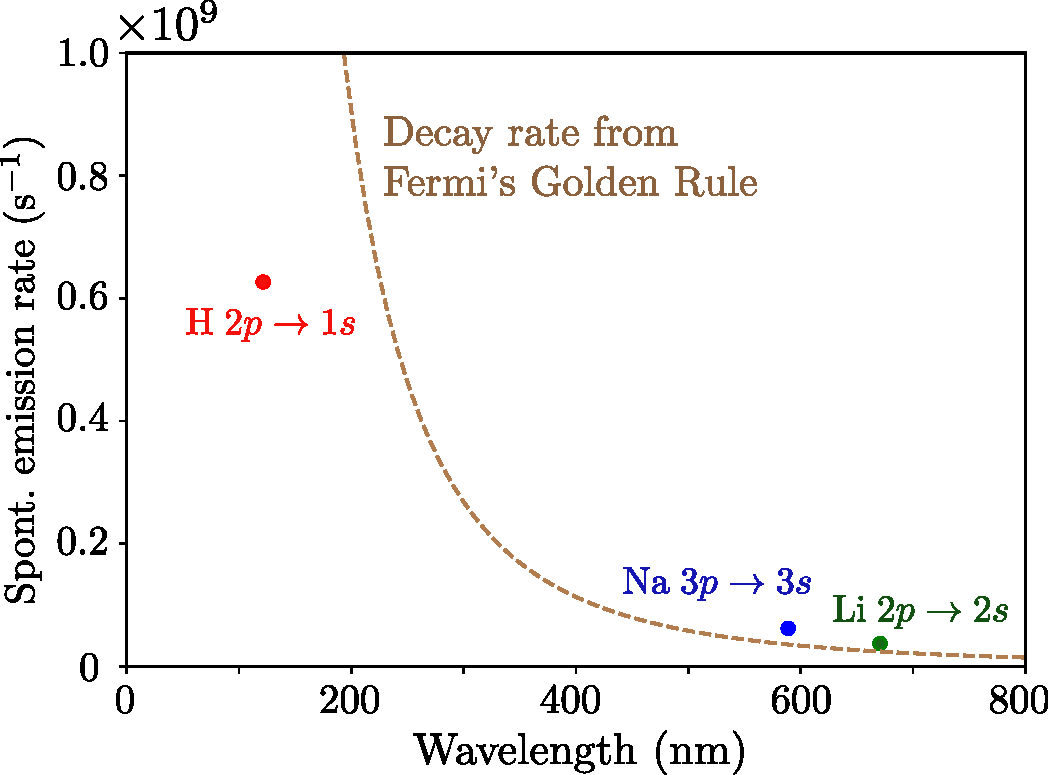
\includegraphics[width=0.53\textwidth]{emissionrates}
  \caption{Spontaneous emission rates (Einstein $A$ coefficients) for
    the $2p\rightarrow 1s$ transition in hydrogen, the
    $2p\rightarrow2s$ transition in lithium, and the $3p\rightarrow3s$
    transition in sodium.  Data points extracted from the NIST Atomic
    Spectra Database
    (\href{https://www.nist.gov/pml/atomic-spectra-database}{https://www.nist.gov/pml/atomic-spectra-database}).
    The dashed curve shows the decay rate based on Fermi's Golden
    Rule, with $|\mathbf{d}| \approx 10^{-10}\,\mathrm{m}$.  }
\end{figure}

%% Need to treat both electrons and photons on the same footing, with QFT
%% language.  Renormalization.

\section*{Exercises}

\begin{enumerate}
\item
  In Section \ref{sec:em_quantization}, we derived the vector
  potential operator, in an infinite volume, to be
  \begin{equation}
    \hat{\mathbf{A}}(\mathbf{r},t) = \int d^3k \sum_{\lambda} 
  \sqrt{\frac{\hbar}{16\pi^3\epsilon_0\omega_{\mathbf{k}}}}\,
  \Big(\hat{a}_{\mathbf{k}\lambda} \, e^{i(\mathbf{k}\cdot\mathbf{r} - \omega_{\mathbf{k}} t)}
  + \mathrm{h.c.}\Big)\, \mathbf{e}_{\mathbf{k}\lambda}.
  \end{equation}
  Since $[\hat{a}_{\mathbf{k}\lambda},
    \hat{a}^\dagger_{\mathbf{k}'\lambda'}] =
  \delta^3(\mathbf{k}-\mathbf{k}') \delta_{\lambda\lambda'}$, the
  creation and annihilation operators each have units of $[x^{3/2}]$.
  Prove that $\hat{\mathbf{A}}$ has the same units as the classical
  vector potential.

\item Repeat the spontaneous decay rate calculation from
  Section~\ref{sec:decay} using the finite-volume versions of the
  creation/annihilation operators and the vector potential operator
  \eqref{Aoperator}.  Show that it yields the same result
  \eqref{alpha}.
  \label{ex:alpha_finite}

\item
  The density of photon states at energy $E$ is defined as
  \begin{equation}
    \mathcal{D}(E) = 2\int d^3k\; \delta(E-E_{\mathbf{k}}),
  \end{equation}
  where $E_{\mathbf{k}} = \hbar c |\mathbf{k}|$.  Note the factor of 2
  accounting for the polarizations.  Prove that
  \begin{equation}
    \mathcal{D}(E) = \frac{8\pi E^2}{\hbar^3c^3},
  \end{equation}
  and show that $\mathcal{D}(E)$ has units of $[E^{-1}V^{-1}]$.
  \label{ex:DE}

\end{enumerate}

\section*{Further Reading}

\begin{enumerate}[[1{]}]
\item F.~J.~Dyson, \textit{1951 Lectures on Advanced Quantum Mechanics
  Second Edition}, arxiv:quant-ph/0608140. [\href{https://arxiv.org/abs/quant-ph/0608140}{link}]
\label{cite:dyson}

\item A.~Zee, \textit{Quantum Field Theory in a Nutshell} (Princeton
  University Press, 2010).
\label{cite:zee}

\item P.~A.~M.~Dirac, \textit{Quantized singularities in the electromagnetic field}, Proceedings of the Royal Society (London) \textbf{133}, 60 (1931).
  \label{cite:monopole}

\item L.~L.~Foldy and S.~A.~Wouthuysen, \textit{On the Dirac Theory of
  Spin $1/2$ Particles and Its Non-Relativistic Limit}, Physical
  Review \textbf{78}, 29 (1950). [\href{https://journals.aps.org/pr/abstract/10.1103/PhysRev.78.29}{link}]
\label{cite:foldy}
\end{enumerate}

\end{document}


%% For decades after the discovery of quantum mechanics, the quantum
%% double-slit experiment was just a ``thought experiment'', meant to
%% illustrate the features of quantum mechanics that had been uncovered
%% by other, more complicated experiments.  Nowadays, the most convenient
%% way to do the experiment is with light, using single-photon sources
%% and single-photon detectors.  Quantum interference has also been
%% demonstrated experimentally using electrons, neutrons, and even
%% large-scale particles such as buckyballs.
